%% LaTeX2e class for student theses
%% thesis.tex
%% 
%% Karlsruhe Institute of Technology
%% Institute for Program Structures and Data Organization
%% Chair for Software Design and Quality (SDQ)
%%
%% Dr.-Ing. Erik Burger
%% burger@kit.edu
%%
%% See https://sdq.kastel.kit.edu/wiki/Dokumentvorlagen
%%
%% Version 1.4, 2023-06-19

%% Available page modes: oneside, twoside
%% Available languages: english, ngerman
%% Available modes: draft, final (see README)
\documentclass[twoside, english]{sdqthesis}

%% Todonotes package
\usepackage[obeyFinal]{todonotes}
\setuptodonotes{inline}
\setuptodonotes{inlinewidth=0.95\linewidth}

%% Nowidow package
\usepackage[defaultlines=3,all]{nowidow}

%% Subcaption package required for subfigures
\usepackage{subcaption}

%% Glossaries package required for acronym section
\usepackage[acronym,toc,section=chapter,numberedsection=false,style=listgroup]{glossaries}
\makeglossaries
\loadglsentries{sections/acronyms.tex}

%% Cleveref package
\usepackage{cleveref}

\usepackage{amsmath}

\usepackage{algorithm}
\usepackage{algpseudocode}
\algrenewcommand\algorithmiccomment[1]{//~#1}
\newcommand*\LineComment[1]{\State //~#1}
\newcommand*\ForIn[2]{\ForAll{#1 $\in$ #2}}
\newcommand*\Let[2]{\State #1 $\gets$ #2}

%% ---------------------------------
%% | Information about the thesis  |
%% ---------------------------------

%% Name of the author
\author{Moritz Gstür}

%% Title (and possibly subtitle) of the thesis
\title{Certificateless Attribute-Based Server-Aided Cryptosystem for Substation Automation Systems (CASC-SAS)}

%% Type of the thesis 
\thesistype{Master's Thesis}

%% Change the institute here, ``KASTEL'' is default
\myinstitute{Institute for Automation and Applied Informatics (IAI)}

%% You can put a logo in the ``logos'' directory and include it here
%% instead of the SDQ logo
% \grouplogo{myfile}
%% Alternatively, you can disable the group logo
\nogrouplogo

%% The reviewers are the professors that grade your thesis
\reviewerone{Prof. Dr. Veit Hagenmeyer}
\reviewertwo{Prof. Dr. Achim Streit}

%% The advisors are PhDs or Postdocs
\advisorone{Dr. Mohammed Ramadan}
%% The second advisor can be omitted
\advisortwo{Dr.-Ing. Ghada Elbez}

%% Please enter the start end end time of your thesis
\editingtime{01. August 2024}{03. February 2025}

\settitle

%% --------------------------------
%% | Bibliography                 |
%% --------------------------------

%% Use biber instead of BibTeX, see README
\usepackage[citestyle=numeric,style=numeric,sorting=none,maxcitenames=2,backend=biber]{biblatex}
\addbibresource{../bibliography/masterthesis.bib}

%% ====================================
%% ====================================
%% ||                                ||
%% || Beginning of the main document ||
%% ||                                ||
%% ====================================
%% ====================================
\begin{document}

%% Set PDF metadata
\setpdf

%% Set the title
\maketitle

%% The Preamble begins here
\frontmatter

%% LaTeX2e class for student theses: Declaration of independent work
%% sections/declaration.tex
%% 
%% Karlsruhe Institute of Technology
%% Institute of Information Security and Dependability
%% Software Design and Quality (SDQ)
%%
%% Dr.-Ing. Erik Burger
%% burger@kit.edu
%%
%% Version 1.5, 2024-02-12

\thispagestyle{empty}
\null\vfill
\noindent\hbox to \textwidth{\hrulefill} 
%
% Gemäß Studien- und Prüfungsordnung Bachelor Informatik des KIT,
% § 14 (5) vom 10.05.2022
% 
\iflanguage{english}{I declare that I have developed and written the enclosed
thesis completely by myself. 
I have not used any other than the aids that I have mentioned. 
I have marked all parts of the thesis that I have included from 
referenced literature, either in their original wording or paraphrasing their
contents. 
I have followed the by-laws to implement scientific integrity at KIT.}%
{Ich versichere wahrheitsgemäß, die Arbeit selbstständig verfasst, alle benutzten 
Quellen und Hilfsmittel vollständig und genau angegeben und alles kenntlich gemacht 
zu haben, was aus Arbeiten anderer unverändert oder mit Abänderungen entnommen wurde 
sowie die Satzung des KIT zur Sicherung guter wissenschaftlicher Praxis in der 
jeweils gültigen Fassung beachtet zu haben. }
 
 
%% ---------------------------------------------
%% | Replace PLACE and DATE with actual values |
%% ---------------------------------------------
\textbf{Karlsruhe, 03. February 2025}
\vspace{1.5cm}
 
\dotfill\hspace*{8.0cm}\\
\hspace*{2cm}(\theauthor) 
\cleardoublepage

\setcounter{page}{1}
\pagenumbering{roman}

%% ----------------
%% |   Abstract   |
%% ----------------
 
%% For theses written in English, an abstract both in English
%% and German is mandatory.
%%
%% For theses written in German, a German abstract is sufficient.
%%
%% The text is included from the following files:
%% - sections/abstract

\includeabstract

%% ------------------------
%% |   Table of Contents  |
%% ------------------------
\tableofcontents

\listoffigures
\listoftables

%% -----------------
%% |   Main part   |
%% -----------------

\mainmatter

\chapter{Introduction}
\label{ch:introduction}
Modern Operational Technology (OT) such as Industrial Control Systems (ICS) increasingly rely on Information and Communication Technology (ICT) for monitoring and control~\cite{Stouffer2023}.
As a consequence, the resemblance of OT and Information Technology (IT) systems increases, as OT systems adopt IT technology.
This development leads to new possibilities including the integration of distributed OT into Supervisory Control And Data Acquisition (SCADA) systems.
Nevertheless, new challenges arise from the increased usage of ICT in OT systems.

According to \citeauthor{Stouffer2023} \cite{Stouffer2023}, the typical long life cycle of OT systems and their unique requirements regarding performance, reliability, security, safety, privacy, and environmental impact have to be taken into account when designing, operating, and maintaining OT systems.
In the following, we focus on the information security of OT systems.
Although a variety of information security solutions exist for IT, migration of existing approaches to the OT domain may not be a viable solution due to the differing system characteristics, risks, and priorities.
An example for the differing priorities are information confidentiality and access control.
While the prevention of unauthorized access represents the core objective of IT security approaches, OT systems and especially OT-based critical infrastructures prioritize system availability and reliability.

Within the scope of this thesis, we focus on the occurring communication in a specific type of OT system.
The field of application of the approach proposed by this thesis is known as Substation Automation System (SAS).
A SAS represents the entirety of communication and control equipment of a substation~\cite{Padilla2015}.
A substation is a facility of a high-voltage electricity grid connecting power transmission and distribution lines that use different voltage levels~\cite{oshaSubstation}.
A substation and its SAS represent a specific type of ICS.
The tasks of a SAS are time-critical and have to be executed reliably, as the electricity sector and its substations are critical infrastructures.

The IEC 61850 series provides standards for the communication networks of digital energy systems~\cite{IEC61850P5}.
The goal of the IEC 61850 series is seamless communication and interoperability of systems in a smart energy grid.
Although standards for the communication in a SAS are provided by the IEC 61850 standards, information security is not an objective of these standards.
To overcome this problem, the IEC 62351 standard series was created by the~\citeauthor{IEC62351P6}.
Part 6 of the IEC 62351 series provides standardized security means for communication compliant to IEC 61850~\cite{IEC62351P6}.
Moreover, Part 8 of the IEC 62351 series provides a role-based access control concept for power system~\cite{IEC62351P8}.

\section{Objective}
\label{sec:introduction:objective}
Although standards regarding the communication networks of smart grid systems are widely accepted and utilized, information security continues to confront unresolved challenges.
Historical evidence indicates that economically or politically motivated adversaries pose a risk to OT systems, including energy-related systems.
The \citeauthor{canada2021} \cite{canada2021} published a list of 28 OT-related cybersecurity incidents between 2010 and 2020, including incidents in energy-related sectors.
These incidents comprise 13 state-sponsored incidents, 13 cybercrime incidents, and two incidents perpetrated by thrill-seeking individuals.
The state-sponsored incidents include the Stuxnet malware deployed in Iranian nuclear power and enrichment facilities in 2010 \cite{bbc2010}, the Shamoon malware used against Saudi Aramco in 2012 \cite{reuters2012}, the Blackenergy malware used to attack Ukrainian power distribution systems in 2015 \cite{cisa2021a}, the Industroyer/CrashOverride malware used to shut down remote terminal units of a Ukrainian power transmission facility in 2016 \cite{reuters2016,cisa2021b}, and the Triton/Trisis malware used to attack Triconex Safety Instrumented System (SIS) controllers in 2017 \cite{johnson2017}.
% ...and other incidents in 2013, 2014, 2015, 2017, 2018 as well as 2020 \cite{wsj2015,cisa2018a,bsi2014,hdn2017,vice2017,cisa2018b,toi2020,warrick2020}.

Despite the existence of standards for communication and information security including the IEC 61850 and 62351, there are remaining challenges in order to secure SAS communication.
This thesis focuses on these remaining challenges to enhance the information security of SAS communication.
As stated by \citeauthor{Ishchenko2018} \cite{Ishchenko2018}, these challenges include, among others, ensuring the integrity and authenticity of substation control and protection communication without compromising the time criticality.
For this purpose, cryptographic signature and verification approaches can be employed in the SAS environment.
According to \citeauthor{Elbez2019} \cite{Elbez2019}, the strict time constraints of the low latency communication in substations are key factors for the information security.
Accordingly, asymmetric cryptography formerly specified by the IEC 62351 standards is not appropriate due to computational complexity and latency.

% Based on this proposed approach, the following research questions are going to be answered in the course of this thesis:
Due to an increase in processing performance of IT and OT devices nowadays, this thesis examines the applicability of effective and efficient asymmetric cryptography in substations.
For this purpose, this thesis proposes new cryptographic and cybersecurity approaches for authentication, authorization, and access control.
Moreover, the thesis discusses the employment of speedup techniques to enable the usage of secure asymmetric cryptography in time-critical OT systems.
Therefore, the following research questions are going to be answered in the course of this thesis:
\begin{description}
    \item[RQ1] How can expressive and flexible but yet computationally expensive access control approaches such as Attribute-Based Access Control (ABAC) be employed to enable prevention of unauthorized access, enable the Separation of Duties (SoD), and ensure the Principle of Least Privilege (PoLP) in a time-critical SAS environment?
    \item[RQ2] How can a secure certificateless server-aided public key cryptography approach be designed and implemented, that is able to ensure the authenticity, integrity, and non-repudiation of communication in a time-critical SAS environment?
    \item[RQ3] How can authentication, authorization, and access control be integrated into a malleable, extendable, certificateless, attribute-based, and server-aided cryptosystem for time-critical SAS communication?
\end{description}

\section{Contribution}
\label{sec:introduction:contribution}
With the aim of providing means to enhance the information security in a SAS, we propose a \textbf{C}ertificateless \textbf{A}ttribute-Based \textbf{S}erver-Aided \textbf{C}ryptosystem for \textbf{S}ubstation \textbf{A}utomation \textbf{S}ystems (CASC-SAS).
The main objective of the proposed approach is to provide secure protocols, algorithms, and schemes for SAS communication based on asymmetric cryptography.
% The provided protocols, algorithms, and schemes aim to satisfy SAS security requirements such as integrity, authenticity, and non-repudiation, while taking the strict time constraints of the SAS domain into account.
The provided protocols, algorithms, and schemes aim to satisfy SAS security requirements such as integrity, authenticity, access control, and non-repudiation.
The approach not only aims to enhance the security of SAS communication by satisfying security objectives, but also takes the specific characteristics, risks, and priorities of OT, ICS, and SAS into account.
Our proposed cryptosystem is based on a dual-path four-layered architecture.
Furthermore, the CASC-SAS approach is divided into two core concepts or components.
These two concepts are referred to as CASA and SABAAC.

\subsubsection*{Certificateless Attribute-Based Server-Aided Authentication (CASA)}
CASA is an attribute-based public key approach.
Instead of relying on trusted Certificate Authorities (CA), the approach employs certificateless public key cryptography.
CASA provides cryptographic protocols, algorithms, and schemes that serve as a foundation for cybersecurity approaches in a SAS.
To take the time criticality of SAS communication into account, the approach features server-aided algorithms and online/offline cryptography.

\subsubsection*{Server-Aided Attribute-Based Authorization \& Access Control (SABAAC)}
SABAAC is a server-aided ABAC approach.
The approach uses the provided cryptographic protocols, algorithms, and schemes of CASA as a foundation.
It enables the prevention of unauthorized access to devices of a SAS.
Our approach aims to demonstrate the applicability of access control policies, which are expressive and flexible with regard to the attributes used but yet computationally expensive to evaluate, in an environment with strict time and resource constraints.
For this purpose, SABAAC not only relies on server-aided algorithms, but also provides speedup techniques such as access decision caching and policy evaluation precomputation.

\chapter{Fundamentals}
\label{ch:fundamentals}
The purpose of this chapter is to introduce, define, and describe the fundamental terms and concepts of this thesis proposal.
This chapter provides an introduction for access control in \autoref{sec:accesscontrol}.
Moreover, the relevant fundamentals of asymmetric cryptography are discussed in \autoref{sec:fundamentals:cryptography}.

\section{Attribute-Based Access Control (ABAC)}
\label{sec:accesscontrol}
Access control is the process of granting and denying specific requests to logical or physical services and resources \cite{NIST2022}.
Based on the type of service or resource guarded by the access control, two types of access control can be distinguished.
Physical access control supervises access requests to physical facilities.
Logical access control supervises the access to information and information processing services.
Within the scope of the thesis proposal, the term access control will be used to describe logical access control for IT and OT systems.

Logical access control protects objects like data, services, executable applications, or network devices from unauthorized operations \cite{Hu2014}.
An operation is performed by a subject on a specific object.
To protect an object, its owners establish access control policies.
These policies describe which subjects may perform certain operations on a specific object.
The policies are enforced by a logical component referred to as Access Control Mechanism (ACM) \cite{Hu2014}.
The ACM receives the access request from a subject, decides whether the request should be granted or denied, and enforces the decision taken.
The ACM takes the decision based on a framework called access control model.
The access control model defines the functionalities and environment including subjects, objects, and rules for the ACM to take and enforce a decision.

Attribute-Based Access Control (ABAC) is an access control model enabling access decisions based on attributes associated with subjects, objects, actions, and the environment of a system \cite{JTF2020}.
In other words, in ABAC an access request of a subject to perform operations on an object is decided based on assigned attributes of the subject and object, environment conditions, and a set of policies \cite{Hu2014}.
Within the context of ABAC, an attribute is a characteristic containing information in the form of a name-value pair \cite{Hu2014}.
A subject attribute such as identity, clearance, or department describes the characteristics of a person or non-person entity.
An object attribute such as the object classification, type, or owner describes the resource for which the access is requested.
An operation or action attribute describes the function performed on an object by a subject.
The environment conditions or environment attributes describe the context of an access request.
Environment conditions include dynamic characteristics like time of the day, day of the week, and request location of the subject.

A policy represents a rule based on which an access decision is taken for specific attributes \cite{Hu2014}.
As a consequence, a policy can be seen as a relationship between subject, object, environment, and operation attributes describing under which circumstances the ACM grants or denies an access request.

Role-Based Access Control (RBAC) and Identity-Based Access Control (IBAC) represent special cases of ABAC regarding their attributes used \cite{Hu2014}.
An advantage of ABAC compared to other access control models is the higher flexibility regarding multifactor policy expression.
Moreover, ABAC can take access control decisions based on ad-hoc knowledge and knowledge from separate infrastructure.
This is possible due to ABAC taking decisions at request time by evaluating policies instead of static decision-making as found in IBAC and RBAC.

\section{Asymmetric Cryptography (Public-Key Cryptography)}
\label{sec:fundamentals:cryptography}
Cryptography is a scientific discipline concerned with the study of methodologies, algorithms, schemes, and protocols for the encryption and verification of information~\cite{Barker2016,Barker2020,CNSS2022}.
In other words, cryptography provides means to prevent unauthorized access and to enable the verification of information.
The objective of cryptography is to satisfy specific security goals, including the assurance of confidentiality, integrity, authenticity, and non-repudiation.

A cryptographic system or cryptosystem is a set of cryptographic algorithms~\cite{Menezes1996}.
A cryptosystem comprises sets of valid inputs and outputs as well as required cryptographic keys~\cite{Eckert2023}.
Two important principles for the design of cryptosystems were formulated by \citeauthor{Kerckhoffs1883} and \citeauthor{Shannon1949}.
As stated by \citeauthor{Kerckhoffs1883}, the cryptosystem must not require secrecy and must be able to be known by the adversary without inconvenience~\cite{Kerckhoffs1883}.
According to \citeauthor{Shannon1949}, it shall be assumed that the adversary knows the system being used~\cite{Shannon1949}.
The goal of a cryptosystem is to provide specific cryptographic services such as encryption or verification.
Verification describes the process of proving the integrity, authenticity, or non-repudiation of information~\cite{Boneh2023}.
The verification of information is based on a so-called tag or signature created by a signature algorithm.
Encryption describes the process of transforming plain information called plaintext into an unintelligible form called ciphertext to maintain its secrecy~\cite{Barker2016,Boneh2023}.
The inverse process of encryption is referred to as decryption.

Asymmetric cryptography, also referred to as Public-Key Cryptography (PKC), relies on algorithms which use a pair of two related keys for a cryptographic operation and its inverse operation~\cite{Barker2020,CNSS2022,Eckert2023}.
This pair of related keys consists of a private key and a public key.
The private key must be kept secret.
The public key may be shared without consequences for security, as long as its authenticity and integrity is ensured.
Although the two keys are related, the private key cannot be efficiently derived from the public key.

PKC offers the following advantages over symmetric cryptography~\cite{Barker2020,Eckert2023}:
Firstly, PKC does not require a secure channel or secure protocol to exchange keys.
Secondly, the overall number of required keys using PKC is lower.
Moreover, the number of keys scales linear with the number of communication entities.
For example in a network with $n$ entities, $n$ key pairs or $2n$ keys have to be established.
In the same network, pairwise symmetric cryptography would require $n(n-1)/2$ keys.

Nevertheless, symmetric cryptography has advantages in comparison with asymmetric cryptography~\cite{Barker2020}.
Firstly, symmetric-key algorithms are faster than asymmetric-key algorithms.
Secondly, for a given level of security, symmetric cryptographic keys are shorter.
This reduces the memory and bandwidth requirements for key storage and transmission.

\subsection{Certificateless Public-Key Cryptography}
Certificateless Public-Key Cryptography (CL-PKC) can be seen as an intermediate approach between Identity-Based Public-Key Cryptography (ID-PKC) and certificate-based PKC approaches such as Public Key Infrastructure (PKI)~\cite{AlRiyami2003}.
CL-PKC approaches make use of a Trusted Third Party (TTP) called Key Generating Center (KGC) to generate partial private keys based on an entity's identity and a master key~\cite{AlRiyami2003}.
To obtain the private key, the entity combines the partial private key with a secret value.
Consequently, CL-PKC neither suffers from the key escrow problem nor requires a secure communication channel for the key distribution.
To obtain the public key, the entity generates it based on public parameters and the secret value~\cite{AlRiyami2003}.
Similar to ID-PKC, the public key is not derived from the private key and may therefore exist prior to it.
The only restriction is that the public key and the private key must use the same secret value.

\subsection{Attribute-Based Public-Key Cryptography}
Attribute-Based Public-Key Cryptography (AB-PKC) is a generalization of the ID-PKC concept~\cite{Sahai2005,Goyal2006,Hu2023}.
Attribute-Based Encryption (ABE) combines the principles of ABAC with the concept of PKC.
Therefor, attribute-based policies are integrated into cryptographic algorithms in the form of access structures and attributes.
ABE approaches are classified as either Key-Policy ABE (KP-ABE) or Ciphertext-Policy ABE (CP-ABE), depending on whether the access structure is associated with a key or a ciphertext~\cite{Goyal2006,Bethencourt2007,Hu2023}.
In KP-ABE a secret key is able to decrypt a ciphertext if the attributes of the ciphertext satisfy the key-associated access structure.
Consequently, a data owner cannot control who is able to access the data and has to trust a TTP to issue appropriate keys~\cite{Bethencourt2007}.
In CP-ABE A secret key is able to decrypt a ciphertext if the key-associated attributes satisfy the ciphertext's access structure.
Accordingly, each data owner manages the access control policies for its own data, which makes CP-ABE more flexible and scalable than KP-ABE.
Similar to the concept of ABE, Attribute-Based Signatures (ABS) enable the integration of attributes into signing and verification algorithms~\cite{Li2010,Maji2011}.

\chapter{Related Work}
\label{ch:relatedwork}
In the following section, the related work of the thesis is presented.
The introduced related work serves as a foundation for the proposed approach presented in \autoref{ch:approach}.
Moreover, similarities and differences of the related work and the proposed approach are discussed.

The related work consists of two parts.
On the one hand, the first part of the related work introduces means to secure the communication, i.e., frame or packet exchange between devices in a SAS.
For this purpose, we discuss approaches which safeguard the confidentiality, authenticity, integrity, and non-repudiation of SAS communication.
On the other hand, the second part of the related work is dedicated to the prevention of unauthorized access.
Accordingly, we discuss approaches which enable access control and satisfy the Principle of Least Privilege (PoLP) and Separation of Duties (SoD).
% Alternative division: ICT-based security layer/measures (e.g. enc/auth of messages) \& Domain-based security layer/measures (e.g. intrusion detection \& access control)

\section{Secure Communication in Substations}
%%% Ishchenko2018 - Secure Communication of Intelligent Electronic Devices in Digital Substations
An authenticated communication approach for network packets between IEDs and merging units is presented by \citeauthor{Ishchenko2018} \cite{Ishchenko2018}.
They identified the lack of security in existing IEC 61850 substations and ICSs in general as a key weakness.
To mitigate this weakness, \citeauthor{Ishchenko2018} present retrofitting of substations as a viable solution
For this purpose, they introduce a system and bump-in-the-wire device called security filter as an add-on device between IEDs and Ethernet-based communication busses using the Generic Object Oriented Substation Event (GOOSE) or Sampled Values (SV) protocol.
Security filter appends Message Authentication Code (MAC) tags to outgoing messages of the IEDs and verifies incoming MAC tags.
As a consequence, the communication busses are secured against unauthenticated messages achieving the security goals integrity and authenticity.
Moreover, the security filter approach uses a timestamp to avoid replay attacks.

To achieve interoperability with legacy communication systems and compatibility with different substation automation systems, the authors introduce a multimode operation design for the security filter.
The multimode operation design consists of three operation modes.
In filtering mode the security filter verifies all packets incoming packets, blocks compromised packets after a certain threshold, and tags all outgoing packets.
Moreover, the security filter alarms the IED about the compromised packets.
In supervisory mode the security filter tags selected packets based on a specific rate of packets, verifies tagged packets only, and blocks and alarms when the number of compromised packets exceeds the threshold.
Consequently, supervisory mode leads to a reduced computational effort.
The last mode is called advisory mode.
In advisory mode the security filter selectively tags and verifies packets based on a specific rate of packets but only triggers alarms and does not block packets after the threshold of compromised packets is reached.
Additionally, the operation of the security filter can be disabled in case of internal errors allowing all packets to pass through.
\citeauthor{Ishchenko2018} showed that the security filter is able to meet the IEC 61850 performance requirements of GOOSE and SV \cite{IEC61850P5} using a HMAC and GMAC algorithm even on commodity of-the-shelf ARM hardware.

This thesis introduces an approach similar to the security filter approach presented by \citeauthor{Ishchenko2018}.
The architecture and security procedures of the proposed approach are inspired by the security filter.
The concept of authenticated communication is proposed as a foundation for secure communication in substations.
Moreover, the proposed approach aims to extend the employed access control from identity-based to attribute-based authorization.
As a consequence, more complex access control policies can be established within a substation or ICS in general.

%%% Elbez2019 - Authentication of GOOSE Messages under Timing Constraints in IEC 61850 Substations (10.14236/ewic/icscsr19.17)
A review of IEC 62351 security recommendations with regard to message authentication and a comparison of viable authentication approaches for IEC 61850 substations is presented by \citeauthor{Elbez2019} \cite{Elbez2019}.
As stated by the authors, ensuring integrity and authenticity of substation communication is critical.
Similar to the approach presented by \citeauthor{Ishchenko2018}, the authors focus on Ethernet-based substation communication using the GOOSE protocol.
To ensure integrity and authenticity of substation communication, the authors present two authentication schemes for GOOSE messages.
Firstly, the authors present the digital signature authentication approach specified by IEC 62351~\cite{IEC62351P6}.
This approach is based on asymmetric cryptography using the RSA Probabilistic Signature Scheme with Appendix (RSASSA-PSS) algorithm.
Secondly, the authors present a keyed Hash Message Authentication Code (HMAC).
The HMAC approach is based on symmetric cryptography and uses a shared secret for signing and verification of GOOSE messages.
According to the authors, the HMAC approach requires less computation time.
On the one hand, this leads to HMAC being a more viable solution for message authentication under strict timing constraints.
On the other hand, a prior key exchange is required to establish the shared secret for the GOOSE provider and each subscriber.
\citeauthor{Elbez2019} identify the performance of the presented authentication approaches as key factor for GOOSE communication.
As a consequence, the authors implemented the authentication approaches and compared the computational times.
In addition to the presented implementations, computation times from three other papers were taken into account.
According to \citeauthor{Elbez2019}, the presented computational times show that asymmetric cryptography solutions based on RSA and RSASSA-PSS are not suitable for the timing constraints of GOOSE messages.
However, the authentication time of the HMAC approach is of the order of microseconds.
Consequently, as stated by the authors, HMAC is a viable approach for the authentication and integrity protection of GOOSE messages.

This thesis backs the results of the authors by evaluating different cryptographic algorithms for low-latency communication in substations.
While our approach is based on an algorithm-agnostic cryptography concept, the focus of the thesis is on digital signature schemes.
The algorithm-agnostic approach is inspired by the Transport Layer Security (TLS) protocol \cite{rfc8446}.
As a consequence, our approach is based on the idea that not a single cryptographic algorithm should be used, but rather different cryptographic algorithms and schemes might be optimal solutions for different communications in a SAS.
Moreover, our approach emphasizes the advantages of PKC in a SAS, including lightweight and secure key distribution as well as malleability with regard to satisfied security requirements.

%%% Rodriguez2021 - A Fixed-Latency Architecture to Secure GOOSE and Sampled Value Messages in Substation Systems
An authentication and encryption approach for substation communication using the protocols GOOSE and SV is presented by \citeauthor{Rodriguez2021} \cite{Rodriguez2021}.
The authors state that GOOSE and SV messages are sensitive to not only availability and integrity but also confidentiality threats.
Therefore, the authors present a hardware architecture for the encryption and authentication of GOOSE and SV packets at wire-speed conforming to IEC 62351:2020~\cite{IEC62351P6}.
The hardware architecture consists of six sections for packet processing that can be implemented using FPGAs.
According to \citeauthor{Rodriguez2021}, the architecture design follows three main guidelines to face challenges within substations.
Firstly, the architecture has to be modular to support future revisions of standards, algorithms, and protocols.
Secondly, the architecture has to have high performance by making use of techniques like parallelization and pipelining.
Lastly, the implementation in substation systems must be viable with regard to required area usage and computing power.
The authors conducted the evaluation of the presented architecture using simulation-based and hardware-based timing results.
As stated by the authors, the hardware implementation is able to process GOOSE and SV packets with a fixed latency in the order of microseconds.
Consequently, the authors state that the presented hardware architecture is able to provide integrity and confidentiality without exceeding the maximum delivery time of three milliseconds introduced by IEC 61850 for GOOSE and SV packets~\cite{IEC61850P5}.

Besides securing the intra-substation communication based on the GOOSE and SV protocol, the thesis extends the idea of providing integrity, authenticity, and non-repudiation to inter-substation and remote communication.
To achieve flexibility and interoperability with regard to different ICS environments including different protocols and algorithms used, the proposed approach is software-based rather than hardware-based.
Furthermore, the proposed approach does not rely on a symmetric-key algorithms, but rather on asymmetric-key algorithms.
This is possible due to an increase in processing performance of IT and OT devices nowadays.

%%% Hong2019 - Cyber Attack Resilient Distance Protection and Circuit Breaker Control for Digital Substations
According to \citeauthor{Hong2019} \cite{Hong2019}, new technologies in substations lead to benefits including enhanced reliability, interoperability, and reduced engineering effort and costs.
Besides the benefits, new technologies introduce vulnerabilities that may result in security breaches.
As an example, the authors mention unauthorized remote access to substations through misconfigured security devices, such as firewalls.
Moreover, the authors state that an adversary might not only intrude the substation from outside but also from the inside.
From inside the substation, an adversary may inject false measurements into the process bus or gain access to the station bus to inject forged control signals or change the configuration of devices like IEDs.
To protect substations against attacks, \citeauthor{Hong2019} present a domain-based collaborative mitigation approach.
According to the authors, the goal of the approach is to enable substation devices to collaboratively defend against attacks.
For this purpose, the authors propose a distributed security domain layer.
The proposed approach can be employed independently or can complement existing information and communication technology (ICT) security approaches.
As stated by the authors, ICT-based security approaches such as firewalls and intrusion detection systems rely exclusively on ICT domain knowledge, whereas the proposed approach relies on knowledge of the power system domain.
As a consequence, new types of attacks as well as errors caused by substation operators can be detected and mitigated.
\citeauthor{Hong2019} presented three attack scenarios that can be mitigated using the presented domain-based collaborative approach.
The presented attack scenarios are an accidental or malicious IED configuration change, false sensor data injection, and false device command injection.
Collaborating devices can block these attacks by validating sensor data and configuration changes based on measurements and metrics as well as predicting consequences of control actions.

The approach presented in the thesis is inspired by the usage of domain-specific knowledge to detect and block attacks.
The proposed approach uses available domain-specific knowledge to design and implement a substation-specific cryptosystem.
Moreover, the incremental framework of the proposed approach for the system design, threat analysis, and mitigation strategy design is based on the research framework presented by \citeauthor{Hong2019}.

\section{Access Control in Substations}
%%% Ruland2018 - Firewall for Attribute-Based Access Control in Smart Grids (10.1109/SEGE.2018.8499306)
An access control approach driven by ABAC policies for smart grid systems including substations is presented by \citeauthor{Ruland2018} \cite{Ruland2018}.
As stated by the authors, communication security enables information confidentiality and integrity but does not protect against internal attacks.
As a consequence, the authors present an access control approach to protect devices from unauthorized access.
The presented access control approach is realized in the form of an access control firewall.
The presented approach is based on an architecture that implements a split station bus.
The split station bus serves the purpose of controlling access requests from devices of the outer bus to devices connected to the inner bus.
The access control firewall connects the outer and inner station bus by processing access requests of connected devices.
On the one hand, within the scope of substations, devices connected to the outer station bus include Human Machine Interfaces (HMI), station computers, and WAN gateways.
On the other hand, the inner station bus connects IEDs and enables low-latency GOOSE or GSSE communication between them.
The access control firewall enforces access request decisions based on ABAC policies.
The ABAC policies used in the presented approach are defined, communicated, and evaluated using the eXtensible Access Control Markup Language (XACML) standard \cite{Oasis2013}.
According to \citeauthor{Ruland2018}, the access request decisions are made by a Policy Decision Point (PDP) that can either be part of the access control firewall or be implemented as an external server on the outer station bus.

The approach presented in the thesis employs ABAC similarly to the access control approach presented by \citeauthor{Ruland2018}.
Besides employing ABAC to secure the communication between devices on the station bus, the proposed approach controls access requests to any device within the substation that requires access control. 
For this purpose, not a single but rather distributed ABAC firewall is used.
As a consequence, the firewall does not represent a communication bottleneck or single point of failure of an ICS in the proposed approach.

%%% Burmester2013 - T-ABAC: An attribute-based access control model for real-time availability in highly dynamic systems (10.1109/ISCC.2013.6754936)
A real-time capable ABAC approach is presented by \citeauthor{Burmester2013} \cite{Burmester2013}.
The presented approach identifies the requirements of cyber-physical systems including confidentiality, integrity, and availability.
In particular, according to the authors, employing ABAC in real-time availability scenarios can be challenging due to the dynamic and large event space determining the attribute values.
In these real-time availability scenarios, events threatening the system state might not be addressed within strict time limits if attribute values are not available in time.
For this purpose, the authors propose an extended ABAC model that is based on real-time attributes to support availability within the strict time constraints of cyber-physical systems.
A real-time attribute represents an attribute whose value is time-dependent.
The availability of a time-dependent attribute can be expressed with an availability label that is dynamically determined based on user and system events as well as the context of the requested service.
An availability label is referred to as priority if it is associated to a subject attribute, congestion for an object attribute, and criticality for an environment attribute.
The authors demonstrate the real-time ABAC approach for IP multicast in Trusted Computing (TC) compliant networks.
Therefor, the authors propose a congestion control algorithm based on the availability labels.
The proposed algorithm guarantees that high priority packets are delivered timely.
In case of a congestion, lower priority packets may be buffered or dropped to support the real-time requirement of high priority packets.
As stated by the authors, the extended ABAC model is applicable to substation automation systems and medical cyber-physical systems.

The access control policy classification and evaluation presented in the thesis are inspired by the authors' concept of real-time attributes.
In our approach, real-time attributes together with static attributes form dynamic and static ABAC policies, i.e., access control policies whose evaluation does or does not rely on time-variable subject, object, environment, or action attributes.
Consequently, while relying on a similar concept of real-time attributes, the approaches differ in their utilization of these attributes.

%%% Lee2015 - Role-based access control for substation automation systems using XACML (10.1016/j.is.2015.01.007)
An IEC 61850 and IEC 62351 compliant RBAC approach for substations is presented by \citeauthor{Lee2015} \cite{Lee2015}.
According to the authors, data collection and analysis are key drivers in smart grids leading to an increased requirement for data security and access control of substation devices.
To address requirements such as confidentiality and integrity, the authors propose an RBAC approach based on IEC 62351 \cite{IEC62351P8} using XACML \cite{Oasis2013}.
As stated by the authors, the communication within substations can either be classified as session-based TCP/IP client-server communication or Ethernet-based publisher-subscriber communication.
The presented approach focuses on session-based access control for TCP/IP communication on the station bus of substations.
As a consequence, the presented RBAC approach can be employed to process MMS communication between IEDs and devices at station level.
The main contribution of \citeauthor{Lee2015} is an implementation of the presented RBAC approach.
The presented implementation relies on a role-based client-server architecture.
The architecture consists of two interconnected client-server pairs, namely an IEC 61850 client and server as well as a RBAC client and server.
The IEC client sends a request including the client's role to the corresponding IEC server.
The IEC server responds to permitted IEC client requests.
Moreover, the IEC server acts as a Policy Enforcement Point (PEP) by delegating requests to an RBAC client.
The RBAC client transforms an IEC request into an XACML request and sends it to the RBAC server for an access request decision.
The RBAC server serves the purpose of making access request decisions by evaluating access control policies.
An IED of a substation incorporates an IEC 61850 server and RBAC client.
The implementation demonstrates the feasibility of RBAC for substations as specified by IEC 62351~\cite{IEC62351P8}.
Furthermore, as stated by the authors, the presented implementation is capable of processing and responding to MMS requests within the 500 millisecond time requirement for type 3 messages (low speed messages) specified by IEC 61850-5~\cite{IEC61850P5}.

Instead of exclusively relying on roles, the approach presented in the thesis employs ABAC to enable the usage of fine-grained and flexible attribute-based access policies.
Moreover, the goal of the proposed approach is to secure any communication within substations including type 1 messages (fast messages) and type 2 messages (medium speed messages) as described by IEC 61850-5~\cite{IEC61850P5}.

%%% Ma2006 - Constraint-Enabled Distributed RBAC for Subscription-Based Remote Network Services (10.1109/CIT.2006.63)
A distributed RBAC approach for subscription-based remote network services is presented by \citeauthor{Ma2006} \cite{Ma2006a,Ma2006}.
According to the authors, identity management for IBAC is a significant challenge for resource providers and subscribing institutions due to the high number of potential users in subscribing institutions.
Furthermore, traditional RBAC approaches require a centralized administration of roles, users, and resources by a single organization.
As a consequence, traditional RBAC and IBAC approaches do not work well in multi-organization distributed systems such as subscription-based remote network services.
For this reason, \citeauthor{Ma2006} propose an approach called Distributed Role-based Access Control (DRBAC).
DRBAC is a distributed authentication and role-based authorization framework.
As stated by the authors, the distributed authentication is realized by delegating the authentication of users to the corresponding subscribing institutions by issuing authentication delegation certificates.
The subscribing institutions use their existing authentication infrastructure to authenticate users and create digitally signed Service Access Tickets (SAT).
The resource provider is able to use the SAT to verify the legitimacy of requests.
The role-based authorization approach of the DRBAC framework extends traditional RBAC by adding the concept of distributed roles shared by the resource provider and resource subscribers.
The resource provider specifies the distributed roles and exports them to the subscribing institutions via distributed role certificates.
The resource subscribers map their local roles to distributed roles to indirectly associate individual subjects with distributed roles.
Therefore, distributed roles represent a middle layer in the DRBAC framework to abstract from subscriber-specific local roles and individual subject identities.
As a consequence, DRBAC enables access control policies associated with distributed roles rather than subject identities, which leads to an increase in scalability and manageability of access control.
The DRBAC policies are realized in the form of authorization policy certificates.
Each DRBAC policy is associated to a certain distributed role and contains a domain-dependent resource operation permission.
Moreover, the authors state that their DRBAC approach supports temporal, contextual, or cardinality constraints to enhance the semantic expressiveness of access control and enable the definition of higher-level organizational policies.

The authentication and authorization approach employed in the thesis is inspired by the concept of delegation presented by \citeauthor{Ma2006}.
The authors illustrate the concept of delegation within the context of a subscription-based remote network service environment.
The proposed approach entails the utilization of authentication and authorization delegation in substations.
Moreover, the proposed approach elevates the degree of abstraction of the presented delegation concept by decoupling it from the concrete access control model used.
The proposed approach realizes authorization delegation via PDPs that make access control decisions for resource requests in place of other devices.
Furthermore, authentication delegation is used for external resource requests to increase scalability and manageability.

%%% Alcaraz2016 - Policy enforcement system for secure interoperable control in distributed Smart Grid systems (10.1016/j.jnca.2015.05.023)
A rule-based RBAC policy enforcement approach for smart grid systems is presented by \citeauthor{Alcaraz2016} \cite{Alcaraz2016}.
According to the authors, the presented approach integrates into a smart grid system with supernode networking architecture.
As stated by \citeauthor{Samuel2008} \cite{Samuel2008}, supernodes are servers at fixed locations responsible for handling data flows of a set of subscribers.
In other words, supernodes represent proxies enabling peer-to-peer connections between devices of dynamic and heterogeneous networks.
The policy enforcement approach presented by \citeauthor{Alcaraz2016} consists of three execution phases.
The first phase is dedicated to the authentication.
During the authentication phase a subject authenticates itself at an identity server within its own infrastructure.
In case of a successful authentication, the identity server provides the subject with an authentication token.
During the second phase the authorization takes place.
To acquire an authorization token, the Policy Enforcement Point (PEP) of the subject infrastructure provides the authentication token and the desired type of action on the target object to a Policy Decision Point (PDP).
The PDP of the presented approach consists of a validation manager and a Policy Decision Manager (PDM).
The former one validates the authentication token as well as roles and permissions associated with the requesting subject, whereas the latter one evaluates the access request and creates the authorization token if it grants the request.
Moreover, the presented PDM is based on a rule-based expert system and a context manager for the analysis of the subject, target object, and context of the request.   
The last phase of the presented approach is referred to as interoperability.
During the interoperability phase the PEP transparently applies the security policies as indicated by the authorization token and performs the action requested by the subject.

The approach presented in the thesis relies on a system model with an architecture similar to the approach presented by \citeauthor{Alcaraz2016}.
Moreover, the two approaches resemble in their usage of authentication and authorization delegation as well as their awareness regarding the request context realized via PDP decision-making.
Nevertheless, the approaches differ in their degree of dependence on specific access control models.
The approach presented by \citeauthor{Alcaraz2016} depends on the subject-role associations of RBAC for decision-making as specified by IEC 62351-8~\cite{IEC62351P8}.
The proposed approach supports more fine-grained and flexible ABAC policies.

%%% Liu2006 - Study on PMI based access control of substation automation system (10.1109/PES.2006.1709324)
An RBAC-based access control approach using Privilege Management Infrastructure (PMI) for IEC 61850 substations is presented by \citeauthor{Liu2006} \cite{Liu2006}.
The presented access control system is realized in the form of a so-called access security agent component.
According to the authors, the access security agent handles the authentication of subjects, parses role-based privileges from subject attribute certificates, provides certificate storage, and performs cryptographic computing.
Besides the access control system architecture, the authors provide a 1-RTT authentication and attribute certificate exchange protocol relying on symmetric as well as asymmetric cryptography.
Moreover, the authors present an algorithm for access privilege parsing to retrieve roles and access policies from attribute certificates.
In the presented access control approach the parsed role-based access policies are used to establish identity-based access control matrices.
An access control matrix of the presented approach controls the access to logical nodes of a substation IED.
For this purpose, an access control matrix associates subject identities with permitted operations for each individual data object.

In contrast to the approach presented by the authors, our approach relies on attribute-based authorization and access control.
While both approaches aim to secure IEC 61850 substation communication, the thesis is based on a certificateless communication concept.
This concept enables the server-aided evaluation and enforcement of expressive and flexible but yet computationally expensive ABAC policies.
Moreover, we emphasize the importance of securing not only bay level but also station and process level devices of a SAS.

\chapter{Approach}
\label{ch:approach}
In the following section, we introduce our proposed security approach for substation automation systems.
With the aim of securing the time-critical communication between resource-constrained devices in a time-variable environment, we propose a \textbf{C}ertificateless \textbf{A}ttribute-Based \textbf{S}erver-Aided \textbf{C}ryptosystem for \textbf{S}ubstation \textbf{A}utomation \textbf{S}ystems (CASC-SAS).
The CASC-SAS cryptography and cybersecurity approach is able to prevent and mitigate cyberattacks by providing security schemes and mechanisms, and enforcing mandatory communication policies.

The introduction and discussion of the proposed approach is organized as follows.
At the beginning of this chapter in \autoref{sec:approach:system_model}, we discuss the field of application of the proposed approach by introducing a system model and defining its requirements.
Based on the presented system model and requirements, we introduce the CASC-SAS approach in \autoref{sec:approach:casc}.
The two main CASC-SAS concepts, its cryptographic scheme and server-aided access control, are introduced in \autoref{sec:approach:casa} and \autoref{sec:approach:sabac}.
In \autoref{sec:approach:realization} we present the planned realization of the CASC-SAS approach.
Subsequently, we present the proposed evaluation strategies and metrics of the approach in \autoref{sec:approach:evaluation}.
Finally, in \autoref{sec:approach:limitations} we discuss limitations of the proposed approach.
%\todo{Own idea, concept, protocol, evaluation, proof, testing, expected benefits and limitations}
%\todo{SECURITY: Security Goals (CIA + Privacy Preserving)}
%\todo{IDEA: Wrap packages of arbitrary protocols by encripting payload of ethernet package, and adding a new header with ABAC-SS information. Maybe as HW Middleware? If other endpoint does not support the ABAC-SS wrapping fall back to proofing endpoint via identity provider only.}
%\todo{PERF EVALUATION: 1. Run approach on network simulator, and 2. Run approach on raspberry pi's representing different roles like server, DER, user \dots}

\section{System Model}
\label{sec:approach:system_model}
In the following sections, we introduce the system model of the CASC-SAS approach.
The system model serves the purpose of delimiting the scope and area of application of the proposed approach.

The area of application of the proposed approach consists of ICSs in the power system domain.
More specifically, the proposed approach is tailored to the communication and control systems of substations in the electricity grid.
The communication and control equipment of an ICS is referred to as secondary equipment.
The entirety of secondary equipment of a substation is referred to as Substation Automation System (SAS) \cite{Padilla2015}.
Although the proposed approach is tailored to the power system domain and substation environment, its main concepts may also be applied to other ICS with similar requirements and constraints.

\subsection{Architecture}
The architecture of the presented system model and SAS respectively is based on the IEC 61850 standard \cite{IEC61850P5}.
The presented system model architecture consists of four layers called network level, station level, bay level, and process level.
The process, bay, and station level represent the internal layers of a SAS architecture.
The SAS architecture containing the process, bay, and station level as well as the station and process bus further discussed in \autoref{sec:approach:system_model:communication} is shown in \autoref{fig:substation_architecture}.
The network level represents a SAS-external layer to integrate multiple SAS instances and supervisory controllers into a comprehensive power system.
Each of the four layers consists of different devices and provides different control and automation functions:
\begin{enumerate}
    \item Process Level: The process level provides functions to interact with the physical process via sensors and actuators.
    As a consequence, SAS devices located at the process level provide interfaces to the physical process.
    In other words, devices located at the process level transform analog measurement signals or control signals into digital values and vice versa.
    Devices restricted to the transformation and provision of measurement and control values are referred to as Merging Units (MU).
    Moreover, IEDs can be employed to combine MU functions with higher-level functions such as protection or communication tasks.

    \item Bay Level: The bay level provides common functions of so-called bays of a SAS.
    As stated by the \citeauthor{IEC61850P5} \cite{IEC61850P5}, a bay represents a closely connected subpart of a substation with common functionality.
    The devices at bay level supervise the operation of lower-level devices of a SAS bay.
    Consequently, a supervising bay level device is referred to as bay controller or bay protection.

    \item Station Level: The station level provides functions related to the substation as a whole.
    Therefore, the station level comprises devices required for on-site and remote monitoring and control of the substation.
    Devices at the station level include Human Machine Interfaces (HMI) for substation operators as well as Wide Area Network (WAN) gateways like SCADA RTUs.

    \item Network Level: The network level provides higher-level functions exceeding the scope of a single SAS.
    The network level devices include supervisory monitoring and control devices like SCADA MTUs.
\end{enumerate}
\begin{figure}
	\centering
	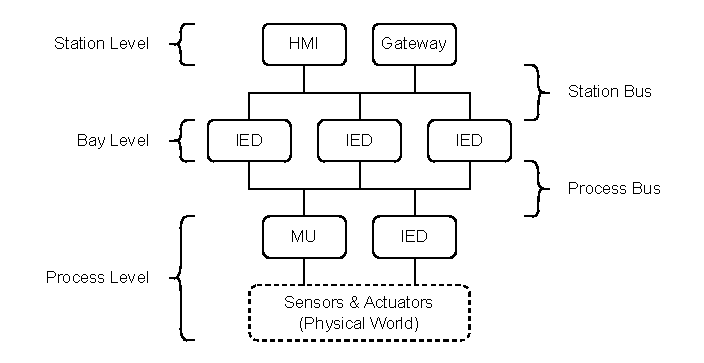
\includegraphics[width=1.0\linewidth]{figures/substation_architecture.drawio.pdf}
	\caption{The internal SAS architecture consisting of three layers called system level, bay level, and process level which are connected via station bus and process bus.}
	\label{fig:substation_architecture}
\end{figure}

\subsection{Communication}
\label{sec:approach:system_model:communication}
In the following, we discuss the communication between devices of the presented system model.
For this purpose, we identify different communication characteristics based on which communication relationships and messages can be classified.
Moreover, we define three messages types for time-critical ICS and SAS communication.
Furthermore, we discuss the bus-based device interactions occurring in the above-mentioned four layer system model.

\subsubsection{Classification Characteristics}
The communication relationships between devices can be classified using different communication characteristics.
Topological communication characteristics can be used to classify the device relationships based on their relative or absolute location within the system model.
Accordingly, communication can either occur between devices on the same layer or different layers of the system model.
Communication on the same layer of the system model is referred to as horizontal communication, whereas communication between devices on different layers is referred to as vertical communication.
Moreover, communication can occur between devices of the same or different subsystems.
Communication between devices of the same subsystem is classified as (subsystem) internal communication, whereas communication relationships including an external device are classified as (subsystem) external communication.
Furthermore, a communication relationship is not limited to a single receiver (unicast) but rather a group of devices (multicast) or all devices (broadcast) may receive a sender's message.

Besides the topology-based classification, communication relationships can be classified based on their continuity.
Continuous, session-oriented, or stateful communication requires an initial session establishment between the involved devices.
While the first message exchange requires additional initialization overhead, subsequent latencies might benefit from the established communication session.
Discontinuous, message-oriented, or stateless communication enables communication without initial overhead for the involved devices.
Consequently, discontinuous communication does not lead to latency emerging from session initialization and management.

Since communication in ICS and SAS is time-critical, communication relationships can be classified based on their communication latency constraints.
Within the scope of the proposed approach, we define communication latency as sum of processing times and transmission times required to exchange information between involved devices.
The transmission time is the time required to transmit a message over a network link with a specific throughput.
The processing time represents the time required for a device to send, forward, or receive a message or packet.
For intermediate network devices like routers and switches the processing time depends on queuing delay and forwarding delay.
For the sender and receiver of a message or packet the processing time consists of enqueue and dequeue delays, cryptographic overhead, and message coding.
As a consequence, the communication latency represents the time required for a message from being put into the sending buffer at the sender to the point when the message is taken from the receiving buffer at the receiver.

\subsubsection{Message Types}
The defined message types of the presented system model are based on the classification characteristics defined above and on the message types and performance classes of the IEC 61850 standard \cite{IEC61850P5}.
The defined message type as well as their typical communication topology, continuity, and latency constraints are shown in \autoref{tab:message_types}.

The low latency message type corresponds to the IEC 61850 \cite{IEC61850P5} message types 1A and 4.
The low latency messages are used for SAS-internal exchange of sampled values and state values.
In IEC 61850 compliant substations the sampled values are exchanged using the Sampled Values (SV) protocol between MUs and IEDs (vertical) or between MUs (horizontal).
Moreover, state values and state changes are exchanged horizontally between IEDs using the Generic Object Oriented Substation Events (GOOSE) protocol.

The medium latency message type corresponds to the IEC 61850 message types 1B and 2.
The medium latency messages are used for internal and external as well as horizontal and vertical session-based client-server communication.
In IEC 61850 substations IEDs use the Manufacturing Message Specification (MMS) protocol to communicate with other IEDs and higher-level devices.

The high latency message type corresponds to the IEC 61850 message types 3 and 5.
This message type is used for HMI interactions as well as non-time-critical operations like file transfers.
In IEC 61850 substations MMS as well as SCADA protocols are used for high latency communication.
\begin{table}
    \centering
    \caption{Message types of the presented system model classified with regard to their topology, continuity, and latency constraints of the communication relationships.}
    \label{tab:message_types}
    \begin{tabular}{l c c c c c}
    \toprule
    \multicolumn{1}{c}{Message Type} & \multicolumn{3}{c}{Topology} & Continuity & Latency\\
    & Externality & Verticality & Receiver & & Constraint\\
    \midrule
    Low Latency & Internal & Horiz./Vert. & Multicast & Message-Based & 3 ms\\
    Medium Latency & Int./Ext. & Horiz./Vert. & Unicast & Session-Based & 20-100 ms\\
    High Latency & Int./Ext. & Horiz./Vert. & Unicast & Session-Based & 500 ms\\
    \bottomrule
    \end{tabular}
\end{table}

\subsubsection{Communication Buses}
The presented system model uses a bus-based approach for SAS-internal message exchange between the system architecture layers.
The implementation of SAS-internal buses is typically based on Ethernet and open or proprietary fieldbus technology.
The bus-based approach as well as the two concrete buses introduced in the following are based on the IEC 61850 standard \cite{IEC61850P5}.

The first bus for SAS-internal message exchange is referred to as process bus.
The process bus is located between the bay level and the process level.
The process bus is used for time-critical message-based publisher-subscriber communication.
GOOSE and SV are the IEC 61850 protocols used for process bus communication.

The second bus for SAS-internal message exchange is referred to as station bus.
The station bus is located between the station level and the bay level.
The station bus connects IEDs at the bay level with each other as well as with gateways and interfaces at the station level.
The communication at the station bus is typically session-based unicast communication with less strict time requirements compared to the process bus.

SAS-external message exchange between devices on the station level and network level use WAN telecommunication technologies including Internet, satellite, cellular, and radio technology.
Secure tunneling approaches like Virtual Private Networks (VPN) can be used to enhance the security of SAS message exchange over an unsecure communication medium.

%\subsection{Threats}
%\todo{System Threats + Adversaries + Attack Trees}

\subsection{Requirements}
In the following, we introduce the requirements of the presented system model.
Based on the identified requirements, functional and non-functional characteristics of the proposed approach are derived and evaluated.
Each system model requirement is associated with a requirement category.
We define five requirement categories for the introduced system requirements.
The requirement categories include security (RQ.SEC), safety (RQ.SAFE), availability (RQ.AVA), performance (RQ.PERF), and interoperability (RQ.INT).
\todo{Add forward/backward secrecy and more.}

%\subsubsection{Security}
\paragraph{RQ.SEC.1 Confidentiality}
The system prohibits unauthorized access to sensitive information stored on devices and payload of messages exchanged within the system and between systems \cite{Eckert2023}.
\paragraph{RQ.SEC.2 Integrity}
The system detects unauthorized manipulation of stored and exchanged data \cite{Eckert2023}.
\paragraph{RQ.SEC.3 Authenticity}
The system can proof the authenticity and trustworthiness of subjects and data objects present in the system \cite{Eckert2023}.
\paragraph{RQ.SEC.4 Non-Repudiation}
The system ensures that a subject cannot dispute its authorship of data and requests \cite{Eckert2023}.
\paragraph{RQ.SEC.5 Least Privilege Principle (PoLP)}
The system ensures that each subject has the least number of privileges necessary to perform its function \cite{JTF2020}.
\paragraph{RQ.SEC.6 Separation of Duties (SoD)}
The system ensures that no subject has enough privileges to be able to misuse the system without collusion \cite{JTF2020}.
\paragraph{RQ.SEC.7 Privacy-Preservation}
\todo{TODO: Does this conflict with the idea of proofing the origin of a request? In other words, is it possible to check if the subject who requested the access decision is still the same subject who used it in its request?}

%\subsubsection{Safety}
\paragraph{RQ.SAFE.1 Safe Operation}
\paragraph{RQ.SAFE.2 Fail-Safe}

%\subsubsection{Availability}
\paragraph{RQ.AVA.1 Continuing Operation}
\paragraph{RQ.AVA.2 Fail-Operational}

%\subsubsection{Performance}
\paragraph{RQ.PERF.1 Communication Latency}
\paragraph{RQ.PERF.2 Computational Complexity}
\paragraph{RQ.PERF.3 Energy \& Power Saving}

%\subsubsection{Interoperability}
\paragraph{RQ.INT.1 Compatibility}
\paragraph{RQ.INT.2 Interchangeability}

\section{Certificateless Attribute-Based Server-Aided Cryptosystem for Substation Automation Systems (CASC-SAS)}
\label{sec:approach:casc}
\subsection{Security Architecture}
\todo{Architecture: CASC-SAS Components \& Layers \& Busses}
\subsubsection{Layers \& Buses}
\subsubsection{Components}
\subsubsection{Stakeholders}

\subsection{Security Policies}
\todo{Security Policies -> Link to Requirements \& Attacks}

\section{Certificateless Attribute-Based Server-Aided Authentication (CASA)}
\label{sec:approach:casa}
In the following section, we present the \textbf{C}ertificateless \textbf{A}ttribute-Based \textbf{S}erver-Aided \textbf{A}uthentication (CASA) concept.
CASA is a certificateless public key cryptography (CL-PKC) approach.
The goal of CASA is to provide cryptographic algorithms and schemes for key generation, key distribution, key revocation, signing, and verification.
Moreover, the goal of CASA is to enable and support more abstract cybersecurity mechanisms like authorization and access control of the CASC-SAS approach.
Therefore, CASA represents the foundation of the employed CASC-SAS cybersecurity mechanisms.

As stated by \citeauthor{AlRiyami2003} \cite{AlRiyami2003}, CL-PKC can be seen as an intermediate approach between certificate-based PKC approaches like Public Key Infrastructure (PKI) and Identity-Based PKC (ID-PKC).
On the one hand, Certificate-based PKC approaches like PKI use a Trusted Third Party (TTP) called Certificate Authority (CA) to issue and store digital certificates.
These digital certificates are used to verify that a certain public key belongs to a specific subject which holds the corresponding private key.
On the other hand, ID-PKC approaches allow the derivation of public keys from subject identities.
The concept of identity-based cryptosystems and schemes was initially proposed by \citeauthor{Shamir1985} \cite{Shamir1985}.
As a consequence, the existence of a public key no longer depends on the existence of a corresponding private key.
Moreover, no certificates are required to verify that a public key belongs to a certain subject, since the subject identity is used to derive the public key.
Nevertheless, in ID-PKC a TTP called Private Key Generator (PKG) is used to generate private keys for subjects based on a system-wide master key.
This leads to key escrow and allows a misbehaving PKG to decrypt confidential messages and forge subject's signatures.

Since CASA is a CL-PKC approach, neither certificates nor key escrow is required.
As proposed by \citeauthor{AlRiyami2003} \cite{AlRiyami2003}, CL-PKC approaches like CASA make use of a TTP called Key Generating Center (KGC) to generate partial private keys for entities based on the entity's identity and a master key.
In order to generate the private key, the entity combines the partial private key with a secret value.
Consequently, the KGC has no access to the private key and no secure channel is required for the key distribution.
According to \citeauthor{AlRiyami2003}, the public key is generated by the entity based on system-wide public parameters and the secret value.
Moreover, the CASA approach proposes a key generation that is not only based on subject identities but rather enables public keys and private keys based on arbitrary attributes of subjects or even groups of subjects.

The key generation of the CASA approach is based on an alternative CL-PKC key generation technique proposed by \citeauthor{AlRiyami2003}.
The defining characteristics of the alternative key generation is the derivation of partial private keys from public keys and identities.
As a consequence, an entity has to generate its public key before it can request a partial private key from the KGC.
This alternative key generation enables sending of partial private keys over unsecure channels and reduces the required trust in the KGC.
Furthermore, this technique allows only one public key to be created for a specific private key.

\subsection{Server-Aided Cryptography}
As PKC mechanisms may consist of computationally complex algorithms and operations such as bilinear pairing, we propose a server-aided PKC approach.
Therefor, we propose an extension of the CL-PKC concept and schemes to make time-critical steps server-aided.
In order to make CASA server-aided, an Untrusted Cryptography Server (UCS) supports devices by handling computationally expensive algorithms instead of executing them locally on resource-constraint devices.
To minimize the required trust, the UCS may only handle certain computations, i.e., partially sign or verify a request of a device.
This server-aided approach enables resource-constraint devices to apply secure algorithms and schemes of CASA in a time-critical OT environment.
In the following, we employ the concept of server-aided PKC for the verification process.

As stated by \citeauthor{Wu2008} \cite{Wu2008}, a server-aided verification process has to satisfy the property of being computation-saving.
A server-aided verification process $V_{Aided}$ is computation-saving if the computational costs for the verifier are strictly less than the costs of non-server-aided verification $V_{Conventional}$.
In other words, $V_{Aided}$ is computation-saving if the equation $Cost(V_{Aided}) < Cost(V_{Conventional})$ holds.

\subsection{Online \& Offline Cryptography}
Since CASA is tailored for time-critical communication, the approach aims to reduce the required time for cryptographic algorithms.
In addition to server-aided cryptography, this time reduction is achieved by precomputation.
For this purpose, each step of an algorithm is classified as either online or offline.
Online steps depend on the sender's public key, the digital signature, or the message.
Consequently, online steps cannot be precomputed.
Nevertheless, specific online steps can be accelerated via server-aided cryptography.
Offline steps depend on information that is available before any message exchange occurs.
Therefore, offline steps can be precomputed to reduce the required time for cryptographic algorithms.

\subsection{Signature Scheme $\mathcal{S}_{CASA}$}
The CASA signature scheme $\mathcal{S}_{CASA} = (I, G_{VAL}, G_{PK}, G_{PPK}, G_{SK}, S, V_{ENT}, V_{SAV}, V_{FIN})$ is a nine-tuple of algorithms.
The algorithms comprise an initialization algorithm $I$, a secret value generation algorithm $G_{VAL}$, a public key generation algorithm $G_{PK}$, a partial private key generation algorithm $G_{PPK}$, a private key generation algorithm $G_{SK}$, a signing algorithm $S$, a partial entity verification algorithm $V_{ENT}$, a partial server verification algorithm $V_{SAV}$, and a final entity verification algorithm $V_{FIN}$.
In the following sections, the specific algorithms are further discussed.

The definition of the CASA signature scheme is based on the definition of digital signature schemes provided by \citeauthor{Boneh2023} \cite{Boneh2023}.
Moreover, since CASA is a CL-PKC approach, the signature scheme is based on the schemes and concepts presented by \citeauthor{AlRiyami2003} \cite{AlRiyami2003} and \citeauthor{Ramadan2023} \cite{Ramadan2023}.
The proposed server-aided verification concept and algorithms are based on schemes proposed by \citeauthor{Ramadan2020} \cite{Ramadan2020}, \citeauthor{Girault2005} \cite{Girault2005} and \citeauthor{Wu2008} \cite{Wu2008}.

\subsubsection{Initialization Algorithm $I$}
The initialization algorithm $(\rho, s) \leftarrow I(\lambda)$ takes the security parameter $\lambda$ as input and outputs the public system parameters $\rho$ and the private master key $s$.
The initialization algorithm is executed by the KGC.
After the execution, $\rho$ is publicly available to all entities, whereas $s$ is only known by the KGC.

\subsubsection{Secret Value Generation Algorithm $G_{VAL}$}
The secret value generation algorithm $\chi_A \leftarrow G_{VAL}(\rho)$ takes the public system parameters $\rho$ as input and outputs the secret value $\chi_A$ of an entity $A$.
The secret value generation algorithm is executed by an entity.
The secret value $\chi_A$ is never shared with other entities and may only be known to entity $A$.

\subsubsection{Public Key Generation Algorithm $G_{PK}$}
The public key generation algorithm $pk_A \leftarrow G_{PK}(\rho, \chi_A, ID_A)$ takes the public system parameters $\rho$, the secret value of an entity $\chi_A$, and the defining attributes of entity $A$ $ID_A$ as input.
The algorithm outputs the public verification key $pk_A$ of entity $A$.
The algorithm is executed by an entity.

\subsubsection{Partial Private Key Generation Algorithm $G_{PPK}$}
The partial private key generation algorithm $ppk_A \leftarrow G_{PPK}(\rho, s, ID_A, pk_A)$ takes the public system parameters $\rho$, the private master key of the KGC $s$, the defining attributes of entity $A$ $ID_A$, and the $A$'s public verification key $pk_A$ as input.
The algorithm outputs the partial private key $ppk_A$ of entity $A$.
The partial private key generation is executed by the KGC on request of an entity.
After the execution, the KGC provides the partial private key to the corresponding entity.

\subsubsection{Private Key Generation Algorithm $G_{SK}$}
The private key generation algorithm $sk_A \leftarrow G_{SK}(\rho, \chi_A, ppk_A)$ takes the public system parameters $\rho$, the secret value of an entity $\chi_A$, and the partial private key $ppk_A$ of entity $A$ as input.
The algorithm outputs the private signing key $sk_A$ of entity $A$.

\subsubsection{Signing Algorithm $S$}
The signing algorithm $\sigma \leftarrow S(sk_A, m)$ takes the private signing key $sk_A$ and message $m$ as input, and outputs the signature $\sigma$.
In other words, the signing algorithm $S$ is used by the sender $A$ of a message $m$ to generate a digital signature $\sigma$.
The generated digital signature $\sigma$ is associated with the message $m$ and the sender's private signing key $sk_A$.
\todo{Introduce Server-Aided Signing Techniques (Server-Partial-Signing, Sender-Signing) and Online/Offline Algorithm Steps.}

\subsubsection{Partial Entity Verification Algorithm $V_{ENT}$}
The partial entity verification algorithm $\sigma_{ENT} \leftarrow V_{ENT}(\rho, pk_A, m, \sigma)$ represents the first step of the server-aided verification process.
The algorithm takes the public system parameters $\rho$, the public verification key $pk_A$ of entity $A$, the message $m$, and the signature $\sigma$ as input.
The algorithm outputs the partially verified signature $\sigma_{ENT}$.
The receiver of a message executes the partial entity verification algorithm $V_{ENT}$ and sends the partially verified signature $\sigma_{ENT}$ to the UCS for server-aided verification.

\subsubsection{Partial Server Verification Algorithm $V_{SAV}$}
The partial server verification algorithm $\sigma_{SAV} \leftarrow V_{SAV}(\sigma_{ENT})$ represents the second step of the server-aided verification process.
The algorithm takes the partially verified signature $\sigma_{ENT}$ as input and outputs the partially verified signature $\sigma_{SAV}$.
The algorithm is executed by the UCS on request of a message receiving entity.
After the execution, the UCS provides the partially verified signature $\sigma_{SAV}$ to the requestor.

\subsubsection{Final Entity Verification Algorithm $V_{FIN}$}
The final entity verification algorithm $\delta \in \{accept, reject\} \leftarrow V_{FIN}(\rho, pk_A, m, \sigma, \sigma_{ENT}, \sigma_{SAV})$ represents the third and last step of the server-aided verification process.
The algorithm takes the public system parameters $\rho$, the public verification key $pk_A$ of entity $A$, the message $m$, the signature $\sigma$, and the partially verified signatures $\sigma_{ENT}$ and $\sigma_{SAV}$ as input.
The algorithm outputs the verification decision $\delta$ which is either $accept$ or $reject$.
In other words, the verification algorithm $V_{FIN}$ is used by the receiver to verify a received message $m$ sent by entity $A$ based on an appended signature $\sigma$.
As $\sigma$ is associated with the message $m$ and the sender's private signing key $sk_A$, it allows the receiver to verify the integrity and authenticity of the received message $m$ using the sender's public verification key $pk_A$.

\subsection{Security Model}
According to the definition of \citeauthor{Boneh2023} \cite{Boneh2023} as well as \citeauthor{Goldwasser1988} \cite{Goldwasser1988}, the proposed signature scheme $\mathcal{S}_{CASA}$ is a secure signature scheme if it is existentially unforgeable under an adaptive chosen-message attack (CMA).
In order to create an existential forgery, i.e., output a valid pair of message and signature for a new message, an adversary carrying out a CMA can request valid signatures from an entity for any message of his choice.
While non-adaptive CMA restricts the adversary to a fixed set of messages chosen prior to the attack, adaptive CMA allows the adversary to request signatures of messages depending on previously obtained signatures.
\citeauthor{Goldwasser1988} describe an adaptive CMA as most powerful attack possible for an enemy restricted to using the signature scheme.

\section{Server-Aided ABAC (SABAC)}
\label{sec:approach:sabac}
\todo{Server-Aided ABAC: is Delegated AC, Distributed Evaluation Strategy (With PDP, Ad-Hoc, Time Variable Attributes), Policies (Rule/Pol Types:RT/Static, DSL, appropriate message types for pol. types), Requests(External, Internal), Protocols, Session-Based via OAT (Estab. channel before comm.), Semi-Delegated Authentication, Delegated Authorization}
% \subsubsection{Delegated Authorization}
% \todo{Policies (Rule/Pol Types:RT/Static, DSL, appropriate message types for pol. types)}
% \todo{Hierarchic PAPs}
% \subsubsection{Semi-Delegated Authentication}
% \todo{Semi-Delegated Authentication}
% \subsubsection{Delegated Authentication}

% \subsubsection{Access Control Protocol}
% \paragraph{Unicast: Client-Server Protocol}
% \paragraph{Multicast \& Broadcast: Publisher-Subscriber Protocol}

\section{Realization}
\label{sec:approach:realization}
\todo{Realization: HW (BITW) or Software Solution}

\section{Evaluation}
\label{sec:approach:evaluation}
\subsection{Evaluation Areas \& Metrics}
\subsubsection{Security Evaluation}
\subsubsection{Performance Evaluation}
\subsubsection{Economic Evaluation}

\subsection{Network Testbed}
\todo{Network Testbed}

\subsection{Network Simulation}
\todo{Network Simulation}

\section{Limitations}
\label{sec:approach:limitations}
\todo{Limitations: No intrusion detection but prevention/mitigation, might not be usable for fast messages, not every crypto for every message type, possible new attack vectors by adding new components, applicability to other ics domains, time protocol interference, physical access control -> future work}

\chapter{Evaluation}
\label{ch:evaluation}
In this section, we analyze and evaluate the CASC-SAS approach and discuss the findings of the evaluation.
The goal of the evaluation is to derive quantitative and qualitative characteristics of the approach.
These characteristics are used to verify the applicability of the approach in the presented field of application, i.e., the employment of the approach in newly constructed or retrofitted substations.
Furthermore, the characteristics are used to identify limitations and future directions of the approach.

\section{Method}
The evaluation is performed theoretically as well as experimentally.
For the theoretical parts of the evaluation, we employ proofs to demonstrate and guarantee certain characteristics of our approach.
The experimentally performed parts of the evaluation are based on a testbed implementation of our approach and the concepts discussed in \autoref{sec:approach:realization}.
The areas and metrics covered by the different parts of the evaluation are discussed in the following section.

\subsection{Evaluation Areas \& Metrics}
The evaluation of our approach is based on the goal-question-metric (GQM) approach \cite{Basili84,Basili92}.
The GQM approach aims to analyze whether an overall goal was achieved by answering a set of questions that represent the different areas of interest of the evaluation.
These questions are answered by deriving and evaluating quantitative and qualitative metrics.
The evaluation of the CASC-SAS approach covers three areas of interest.
The three areas of interest, i.e., questions to be answered, and their corresponding metrics are defined below:
\begin{description}
    \item[Goal:] Protect the time-constrained and traffic-intensive communication of a newly constructed or retrofitted SAS against domain-typical adversaries and attacks.
    \begin{description}
        \item[Question: Security] Does CASC-SAS provide security against typical SAS adversaries and attacks?
        \begin{description}
            \item[Metric:] Which security, safety, and availability requirements can be satisfied by deploying the approach in a SAS?
            \item[Metric:] Which adversary and system characteristics are assumed?
            \item[Metric:] Which attacks can be mitigated, and how can these attacks be mitigated with regard to their corresponding mitigation strategy?
            \item[Metric:] How does the attack surface of the SAS change?
        \end{description}
        \item[Question: Performance] Is CASC-SAS capable of securing time-constrained and traffic-intensive communication of an SAS in an efficient and scalable manner?
        \begin{description}
            \item[Metric:] Which performance requirements can be satisfied by deploying the approach in a SAS?
            \item[Metric:] Which communication characteristics are assumed?
            \item[Metric:] Which message types are supported?
            % \item Resistance against network exceptions including congestion, delay, jitter, duplicated packets, lost packets, and out-of-order packet delivery
        \end{description}
        \item[Question: Compatibility] Is CASC-SAS a viable solution to enhance the security of newly constructed or retrofitted substations?
        \begin{description}
            \item[Metric:] Which compatibility requirements can be satisfied by deploying the approach in a SAS?
            \item[Metric:] Which device requirements are assumed?
            \item[Metric:] What are the additional costs for SAS construction and retrofitting?
            \item[Metric:] Is the approach feasible with regard to SAS retrofitting?
            % \item Cost-benefit efficiency compared to alternative approaches
        \end{description}
    \end{description}
\end{description}

\subsection{Testbed}
To analyze and evaluate the integration of our approach into the SAS architecture, as discussed in \autoref{sec:approach:realization}, we implemented the approach in hardware and software as a testbed.
The software is implemented component-wise using object-oriented high-level programming languages.
The components are primarily implemented using the programming languages Java and Kotlin.
The software implementation of our approach is published open source on GitHub \cite{gitcasc} under the European Union Public Licence (EUPL) \cite{eupl}.
The implementation is divided into three main packages.
These packages, their sub-packages, and the package interrelationships are shown in \autoref{fig:casc_package_structure}.
The common package contains functionalities that are required by all other parts of the implementation.
Among others, the common package contains classes and interfaces related to message ingress and egress, message serialization, concurrency, and cryptography.
The second package and its sub-packages are dedicated to the CASA components and protocols.
The third package and its sub-packages are dedicated to the SABAAC components and protocols.
To avoid circular dependencies between the packages and achieve loose coupling of components, we employ the dependency inversion principle by using interfaces.
\begin{figure}
    \centering
    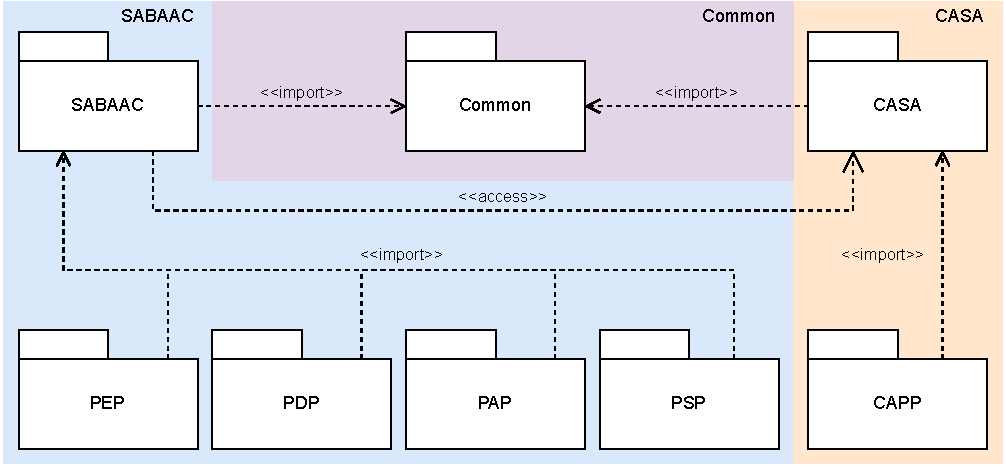
\includegraphics[width=0.9\linewidth]{figures/package_structure.drawio.pdf}
    \caption{Structural package diagram of the CASC-SAS testbed implementation.}
    \label{fig:casc_package_structure}
\end{figure}

To be able to conduct experiments while taking the behavior of physical network communication into account, we transformed the software implementation into a physical system by deploying the SABAAC and CASA components to hardware.
In contrast to deterministic software-based analysis, the testbed evaluation results are practice-oriented and transferable to the SAS domain.
The conceptual topology of our testbed network is visualized in \autoref{fig:evaluation_test_bed}.
The components depicted in blue represent domain-specific devices of an SAS, including IEDs and MUs.
%and computers that mimic the behavior of domain-specific devices of an SAS
The components depicted in yellow represent intermediate network devices for frame and datagram forwarding on the data link layer and network layer.
The components depicted in red are part of the CASC-SAS approach.
The specific hardware used for the experiments is discussed for each experiment individually in the following sections.
\begin{figure}
    \centering
    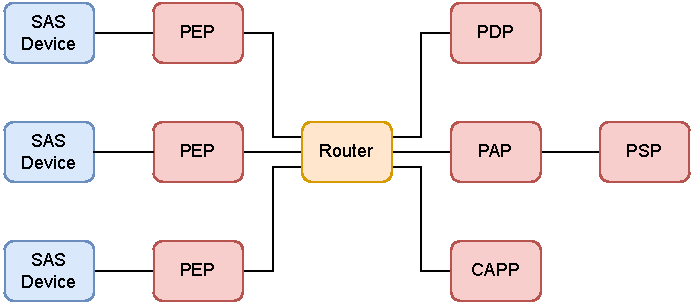
\includegraphics[width=0.8\linewidth]{figures/network_testbed_color.drawio.pdf}
    \caption{Conceptual network topology of the CASC-SAS testbed.}
    \label{fig:evaluation_test_bed}
\end{figure}
%The specific hardware used for the experiments is shown in \autoref{tab:testbed_hardware}.
%We conducted the experiments using a single TTP server that provided the PDP, PAP, PSP, and CAPP services.
%For experiments without real SAS devices, we deployed the PEPs as well as machines that mimic the behavior of domain-specific SAS devices to individual off-the-shelf Raspberry Pi 5 computers.
%For experiments with real IEDs and MUs, only the PEPs were deployed to Raspberry Pi 5 computers.
%
%The simulation and testbed strategy have differing advantages and disadvantages.
%On the one hand, the simulation strategy has the advantage of repeatability and reproducibility due to deterministic behavior, whereas the behavior of the testbed is non-deterministic.

\section{Security Analysis}
In this section, we conduct an analysis of the security of the CASC-SAS approach and its core concepts CASA and SABAAC.
The primary objective of the security analysis is to demonstrate and guarantee certain security-related characteristics of the approach.
As the security analysis is performed theoretically, proofs will be provided demonstrating that the approach is able to mitigate adversarial attacks that endanger these security-related characteristics.
\begin{description}
    \item[Definition.] Unforgeability.\\
    Unforgeability ensures that no adversary can create a valid signature for a message under a policy unless their set of attributes satisfies the policy.
    Unforgeability is defined by using a game between a challenger and an adversary $\mathcal{A}$:
    \begin{itemize}
        \item Setup: The challenger runs the \texttt{Setup} algorithm to generate the public parameters $PK$ and the master secret key $MSK$.
        The public parameters are given to $\mathcal{A}$, while the $MSK$ is kept secret.

        \item KeyGen: $\mathcal{A}$ can query the \texttt{KeyGen} oracle to obtain private keys for sets of attributes of its choice.
        The challenger responds with the corresponding private keys.

        \item SignQueries: $\mathcal{A}$ can request signatures for messages and policies from the \texttt{Sign} oracle.
        The oracle returns valid signatures if the queried attributes satisfy the signing policy.

        \item Forgery: $\mathcal{A}$ outputs a forged signature $(M^*, T^*, \sigma^*)$ for a message $M^*$ and policy $T^*$.
        $\mathcal{A}$ wins if the following conditions hold:
        \begin{itemize}
            \item $\mathcal{A}$ did not request a signature on $(M^*, T^*)$ from the \texttt{Sign} oracle.
            \item $\mathcal{A}$ does not possess a private key whose attributes satisfy the policy $T^*$.
            \item The verification algorithm accepts $\sigma^*$ as a valid signature under $T^*$.
        \end{itemize}
    \end{itemize}

    \item[Definition.] Existential Unforgeability under Chosen-Message Attacks (EU-CMA).\\
    An adversary $\mathcal{A}$ is given access to public parameters, hash oracles, and a signing oracle.
    A scheme is secure if $\mathcal{A}$ cannot forge a valid signature $\sigma^*$ for a new message $M^*$ without knowing the signer's full private key.
    In other words, to create an existential forgery, i.e., create a valid pair of message and signature for a new message, an adversary carrying out a CMA can request valid signatures for any message of his choice \cite{Goldwasser1988}.
    The adversary's advantage in this game is its probability of generating a valid forgery.
    We say the ABS scheme is \textit{existentially unforgeable} if the adversary's advantage is negligible.

    \item[Theorem.] $\mathcal{S}_{CASA}$ is EU-CMA secure under the Computational Diffie-Hellman (CDH) assumption in the random oracle model.\\
    \textit{Proof.} After querying the signing oracle, assume $\mathcal{A}$ forges a signature $\sigma^*$ for $M^*$. The challenger interacts with $\mathcal{A}$ as follows:
    \begin{itemize}
        \item \textit{Setup}: The challenger generates $ppk_i$, $p$, and hash oracles \( H_1, H_2, H_3 \) for \( \mathcal{A} \).
        \item \textit{HashQueries}: The challenger responds to \( H_1, H_2, H_3 \) queries with random values, ensuring consistency.
        \item \textit{SigningQueries}: For $M$ and $\mathsf{Att}_{i}$, the challenger computes:
        \[
        \sigma_i = \big(ppk_{i} \cdot H_3(h)\big)^{\chi_i},
        \]
        where $h = H_2(M || \mathsf{Att}_{i})$.
        \item \textit{Forgery}: If \( \mathcal{A} \) outputs \( \sigma^* \) for \( M^* \), the challenger extracts \( g^{ab} \) from \( g, g^a, g^b \), solving the CDH problem.
    \end{itemize}
    Thus, $\mathcal{A}$'s advantage is negligible under the CDH assumption.
    The $\mathcal{S}_{CASA}$ scheme is secure against EU-CMA attacks.

    \item[Definition.] Collusion Attack.\\
    An adversary $\mathcal{A}$ colludes with a TTP and corrupted signers to derive private keys or forge valid signatures.
    The scheme is secure if such a collusion does not compromise honest signers and does not allow forgery.

    \item[Theorem.] $\mathcal{S}_{CASA}$ resists collusion attacks under the Discrete Logarithm Problem (DLP).\\
    \textit{Proof.} Suppose $\mathcal{A}$ colludes with the CAPP to derive $sk_i = (ppk_i, \chi_i)$, then the following steps are performed:
    \begin{itemize}
        \item The CAPP knows $ppk_i = H_1(\mathsf{ID}_i || \mathsf{ATT}_i)^{s}$.
        \item The signer independently chooses $\chi_i$ and the DLP ensures $\mathcal{A}$ cannot derive $\chi_i$ from $y_i = g^{\chi_i}$.
        \item Without $\chi_i$, $\mathcal{A}$ cannot compute:
        \[
        \sigma_i = \big(ppk_i \cdot H_3(h)\big)^{\chi_i}.
        \]
    \end{itemize}
    Thus, collusion cannot compromise security.
    The $\mathcal{S}_{CASA}$ scheme is secure against collusion attacks.

    \item[Definition.] Message Replay.\\
    To perform a message replay, an adversary captures and repeats the messages exchanged between two or more network devices.
    The adversary aims to inject false data into the system, or disrupt the operation of the network devices.

    \item[Theorem.] CASC-SAS protects SAS devices against message replay attacks.\\
    \textit{Proof.} Suppose two SAS devices, $Alice$ and $Bob$, exchange messages over a network.
    We assume that an adversary $\mathcal{A}$, as introduced in \autoref{sec:approach:attacks}, is able to eavesdrop and replay the messages sent from $Alice$ to $Bob$, and vice versa.
    For the exchange of a message $m$ between $Alice$ and $Bob$, as shown in \autoref{fig:attack_message_replay}, the following steps are performed:
    \begin{itemize}
        \item $Alice$ sends the message $m$ to $Bob$ via $PEP_{Alice}$.
        \item To satisfy the security policies I and IV of CASC-SAS, $PEP_{Alice}$ encapsulates $m$ and a sequence number $seq_m$ in a packet $m' = (Alice, Bob, m, seq_m)$ and signs $m'$ to get $m'' = (m', \sigma_{m'})$.
        \item $PEP_{Alice}$ sends $m''$ to $PEP_{Bob}$ using the network. $PEP_{Bob}$ receives $m''$ from $PEP_{Alice}$, verifies the signature $\sigma_{m'}$, sets the last sequence number received from $PEP_{Alice}$ to $seq_m$, and delivers $m$ to $Bob$.
        \item $\mathcal{A}$ eavesdrops the message exchange, receives $m''$ at the same time as $PEP_{Bob}$, and replays $m''$ to $PEP_{Bob}$.
        \item $PEP_{Bob}$ receives $m''$ from $\mathcal{A}$. As $PEP_{Bob}$ already processed a packet from $PEP_{Alice}$ with sequence number $seq_m$, $m''$ is discarded.
    \end{itemize}
    $\mathcal{A}$ gains no advantage by replaying $m''$, as neither false data is injected into $Alice$ or $Bob$, nor is the operation of $Alice$ or $Bob$ disrupted.
    Thus, SAS devices are protected against message replay attacks.
    \begin{figure}
        \centering
        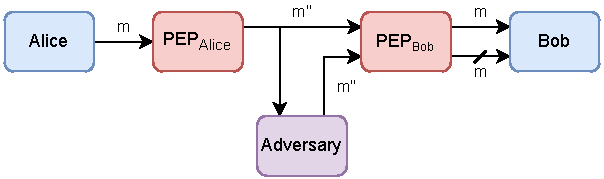
\includegraphics[width=0.75\linewidth]{figures/attack_message_replay.drawio.pdf}
        \caption{Malicious replay of a message exchanged between two PEP-protected SAS devices.}
        \label{fig:attack_message_replay}
    \end{figure}

    \item[Definition.] Message Forgery.\\
    To perform a message forgery, an adversary masquerades as a legitimate device to send malicious messages to other devices.
    By using message forgery, the adversary injects false data into the system, or disrupts the operation of devices.

    \item[Theorem.] CASC-SAS protects SAS devices against message forgery attacks.\\
    \textit{Proof.} Suppose two SAS devices, $Alice$ and $Bob$, exchange messages over a network.
    We assume that only the two devices have the necessary key material to sign and verify exchanged messages.
    As defined in \autoref{sec:approach:attacks}, we assume that an adversary $\mathcal{A}$ is able to initiate arbitrary message exchanges but is unable to bypass or break cryptographic procedures.
    To send a malicious message $m*$ from $\mathcal{A}$ to $Bob$, as shown in \autoref{fig:attack_message_forgery}, $\mathcal{A}$ has to perform the following steps:
    \begin{itemize}
        \item $\mathcal{A}$ creates a message $f$ of its choice.
        \item $\mathcal{A}$ encapsulates $f$ in a packet $m^* = ((Alice, Bob, f, seq_{m^*}), \sigma_{m^*})$, to masquerade as $PEP_{Alice}$.
        \item $\mathcal{A}$ sends $m^*$ to $PEP_{Bob}$.
        \item $PEP_{Bob}$ discards $m^*$ and does not deliver $f$ to $Bob$, as the signature $\sigma_{m^*}$ is not created by $PEP_{Alice}$.
    \end{itemize}
    Since only $PEP_{Alice}$ has the necessary key material to sign messages from $Alice$, $\mathcal{A}$ is unable to masquerade as $Alice$.
    Thus, SAS devices are protected against message forgery attacks.
    \begin{figure}
        \centering
        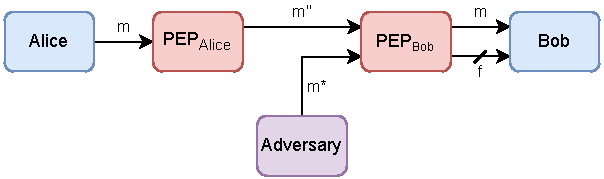
\includegraphics[width=0.75\linewidth]{figures/attack_message_forgery.drawio.pdf}
        \caption{Forgery of a message by masquerading as a PEP-protected SAS device.}
        \label{fig:attack_message_forgery}
    \end{figure}

    \item[Definition.] Message Modification.\\
    To perform a message modification, an adversary captures and alters messages exchanged between two or more network devices.
    Accordingly, message modification is a special type of message forgery that derives a malicious message from a captured message.

    \item[Theorem.] CASC-SAS protects SAS devices against message modification attacks.\\
    \textit{Proof.} Suppose two SAS devices, $Alice$ and $Bob$, exchange messages over a network.
    As with message forgery, we assume that only $Alice$ and $Bob$ have the necessary key material to sign and verify exchanged messages, and that an adversary $\mathcal{A}$ is unable to bypass or break cryptographic procedures.
    We assume that $\mathcal{A}$ performs the attack using a man in the middle approach, i.e., $Alice$ and $Bob$ are not directly connected and the exchanged messages traverse $\mathcal{A}$.
    The modification of a message $m$ from $Alice$ to $Bob$ using a man in the middle approach is shown in \autoref{fig:attack_message_modification}.
    To carry out a message modification attack, $\mathcal{A}$ has to perform the following steps:
    \begin{itemize}
        \item $Alice$ sends the message $m$ to $PEP_{Alice}$.
        \item To satisfy the security policies I and IV of CASC-SAS, $PEP_{Alice}$ encapsulates $m$ and a sequence number $seq_m$ in a packet $m' = (Alice, Bob, m, seq_m)$ and signs $m'$ to get $m'' = (m', \sigma_{m'})$.
        \item $PEP_{Alice}$ sends $m''$ unintentionally to $\mathcal{A}$ using the network.
        \item $\mathcal{A}$ modifies $m$ and encapsulates the modified message $f$ in a packet $m^* = ((Alice, Bob, f, seq_{m}), \sigma_{m})$.
        \item $\mathcal{A}$ sends $m^*$ to $PEP_{Bob}$.
        \item $PEP_{Bob}$ discards $m^*$ and does not deliver $f$ to $Bob$, as the signature $\sigma_{m'}$ does not match the content of $m^*$.
    \end{itemize}
    Since only $PEP_{Alice}$ has the necessary key material to sign messages from $Alice$, $\mathcal{A}$ is unable to renew the signature after modifying the encapsulated message.
    Thus, SAS devices are protected against message modification attacks.
    \begin{figure}
        \centering
        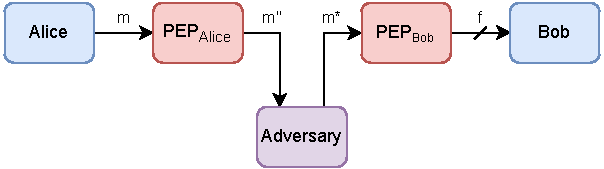
\includegraphics[width=0.75\linewidth]{figures/attack_message_modification.drawio.pdf}
        \caption{Malicious modification of a message exchanged between two PEP-protected SAS devices.}
        \label{fig:attack_message_modification}
    \end{figure}

    \item[Definition.] Time-Delay Attack.\\
    A time-delay attack is the intentional delaying of time-critical messages in a network.
    To perform a time-delay attack, a man in the middle adversary captures a message sent by a network device, and waits a certain time before forwarding it to the message receiver.
    By maliciously delaying exchanged messages, the adversary may either inject outdated data into the system or disrupt the operation of devices.

    \item[Theorem.] CASC-SAS protects SAS devices against time-delay attacks.\\
    \textit{Proof.} Suppose two SAS devices, $Alice$ and $Bob$, exchange messages over a network in the presence of an adversary $\mathcal{A}$, which performs a time-delay attack using a man in the middle approach.
    The performed time-delay attack is shown in \autoref{fig:attack_time_delay}.
    To carry out a message modification attack, $\mathcal{A}$ has to perform the following steps:
    \begin{itemize}
        \item $Alice$ sends the message $m$ to $PEP_{Alice}$.
        \item To satisfy the security policies I and IV of CASC-SAS, $PEP_{Alice}$ encapsulates $m$ with a timestamp-based sequence number $seq_m$ in a packet $m' = (Alice,\allowbreak Bob,\allowbreak m,\allowbreak seq_m)$ and signs $m'$ to get $m'' = (m', \sigma_{m'})$.
        \item $PEP_{Alice}$ sends $m''$ unintentionally to $\mathcal{A}$ using the network.
        \item $\mathcal{A}$ receives $m''$ and waits a certain time before sending it to $PEP_{Bob}$.
        \item $PEP_{Bob}$ discards $m''$ and does not deliver $m$ to $Bob$, as the sequence number $seq_m$ indicates that the packet was maliciously or accidentally delayed.
    \end{itemize}
    The delay of $m''$ would only be unnoticeable if $\mathcal{A}$ was able to update the sequence number.
    However, as only $PEP_{Alice}$ has the necessary key material to sign messages from $Alice$, $\mathcal{A}$ is unable to update the sequence number.
    Thus, SAS devices are protected against time-delay attacks.
    \begin{figure}
        \centering
        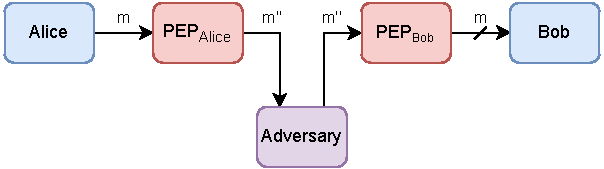
\includegraphics[width=0.75\linewidth]{figures/attack_time_delay.drawio.pdf}
        \caption{Malicious delaying of a message exchanged between two PEP-protected SAS devices.}
        \label{fig:attack_time_delay}
    \end{figure}
    %\item[Theorem.] CASC-SAS protects SAS devices against flooding attacks.\\
    %\textit{Proof.}
\end{description}

\section{Performance Analysis}
In this section, we conduct an analysis of the performance aspects of our approaches CASA and SABAAC.
The objective of the performance analysis is to demonstrate that our approaches are viable solutions to secure message exchanges, taking the strict time and resource constraints of a SAS into account.
For this purpose, we conducted an experimental estimation of message exchange latencies using our testbed implementation and off-the-shelf hardware.
In \autoref{sec:evaluation:performance:setup} the setup of the experiment is discussed in detail.
In \autoref{sec:evaluation:performance:procedure} we describe the procedure and results of the experiment.

\subsection{Experimental Setup}
\label{sec:evaluation:performance:setup}
The testbed of the performance analysis consists of eight devices.
The hardware devices used for the experiment are listed in \autoref{tab:performance_analysis_hardware}.
Two Raspberry Pi 5 were deployed to mimic domain entities that communicate with each other.
Another two Raspberry Pi 5 were used as PEPs protecting the domain entities.
A ThinkPad T480 provided the services of the PAP, PSP, PDP, and CAPP.
\begin{table}
    \centering
    \small
    \caption{Hardware used for the performance analysis testbed.}
    \label{tab:performance_analysis_hardware}
    \begin{tabular}{c c c c}
    \toprule
    Manufacturer & Device & Task & Amount\\
    \midrule
    % SAS Devices
    TP-Link & Omada ER605 & Gigabit Router & 1\\
    % CASA & SABAAC
    Raspberry Pi Ltd & Raspberry Pi 5 8GB & PEP \& Domain Entity & 4\\
    Lenovo & ThinkPad T480 & PDP/PAP/PSP/CAPP & 1\\
    Bechtle & ARTICONA Adapter & USB-A to RJ45 Adapter & 2\\
    \bottomrule
    \end{tabular}
\end{table}

The network topology of the devices used for the performance analysis is shown in \autoref{fig:performance_analysis_topology}.
The PAP, PSP, PDP, CAPP, and PEPs were connected to an industrial grade TP-Link Omada router using Ethernet over twisted-pair.
Each domain entity was connected to its corresponding PEP using Ethernet over twisted-pair, i.e., by using the on-board RJ45 Ethernet connector of the Raspberry Pi 5 domain entity.
However, since the Raspberry Pi 5 only possesses a single on-board RJ45 Ethernet connector, an additional USB-A to RJ45 Ethernet adapter had to be used for both PEPs in order to connect them to the router and to the domain entities.
\begin{figure}
    \centering
    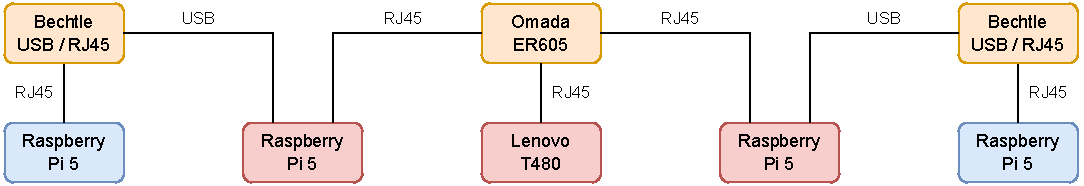
\includegraphics[width=1.0\linewidth]{figures/performance_evaluation_topology.drawio.pdf}
    \caption{Network topology of the performance analysis testbed.}
    \label{fig:performance_analysis_topology}
\end{figure}

\subsection{Procedure \& Results}
\label{sec:evaluation:performance:procedure}
To demonstrate the viability of our approach with regard to securing time critical message exchanges, we aimed to evaluate the extent to which our approach was capable of handling different message types.
For this purpose, we conducted an experiment to estimate the end-to-end communication latency of a message exchange between two domain entities.
The three message types that were considered for the evaluation are discussed in \autoref{sec:approach:system_model:communication:message_types} and listed in \autoref{tab:message_types}.

We realized the message exchange latency estimation by implementing a benchmark program and deploying it to the domain entities.
The benchmark program was implemented in Python.
The program is published open source on GitHub \cite{gitcasc} alongside the implementation of our approach.
The program estimated the end-to-end latency between the two domain entities based on the RTT of a bidirectional message exchange.
We chose UDP as a message exchange protocol for the experiment in order to avoid external latency influences, such as the flow control and congestion control of the Transmission Control Protocol (TCP).
To measure the RTT, the so-called active benchmark entity sent a timestamp to the passive benchmark entity.
The passive entity replied to the message with the received timestamp.
Thus, after receiving the response from the passive entity, the active entity was able to calculate the RTT by subtracting the received timestamp from the current timestamp.
As a consequence, no time synchronization was required between the domain entities.
Furthermore, under the assumption of symmetric transmission times, the accuracy of the RTT measurements only depended on the accuracy of the active entity's system clock.
To avoid RTT fluctuations or an offset caused by the router's buffering and forwarding strategy, messages were sent sequentially, i.e., the active entity waited for the arrival of a response before sending another timestamp message.

The procedure of the experimental latency estimation consisted of ten key events.
The sequence of events and the corresponding messages exchanged between the devices are shown in \autoref{fig:performance_analysis_latency_steps}.
To improve the readability of the shown message exchanges, the USB-A to RJ45 Ethernet adapters were omitted from the figure.
The steps of the experiment procedure are defined in the following:
\begin{description}
    \item[Step 1: Send Request]~\\
    At the initial state of the experiment, no domain-specific messages were exchanged between the devices.
    The necessary key material for signing and verification was already exchanged prior to the experiment.
    The PDP used the precomputed evaluation strategy for access policies, i.e., the access decisions were periodically refreshed and cached.
    The PEPs used a hybrid access decision evaluation strategy, i.e., access decisions were requested and cached as soon as they were needed.
    To initiate the end-to-end latency estimation, the active domain entity sent a UDP packet with its current system clock timestamp to the passive domain entity.

    \item[Step 2: Request Access]~\\
    As the active entity was protected by a PEP, the outgoing UDP packet was captured by the active entity's PEP.
    The PEP checked if an applicable and valid access decision for the packet-related data frames was available in its cache.
    If no applicable or valid access decision was available, the PEP sent an access request to the PDP.

    \item[Step 3: Exchange Request Payload]~\\
    As soon as an applicable and valid access decision was available, the active entity's PEP processed the UDP packet as discussed in \autoref{sec:approach:sabaac:accesscontrol} and sent a payload exchange request to the passive entity's PEP.

    \item[Step 4: Forward Request]~\\
    On receipt of a payload exchange request, the passive entity's PEP verified the request.
    After the request verification, the contained UDP packet was forwarded to the passive domain entity.

    \item[Step 5: Send Response]~\\
    On receipt of the UDP packet, the benchmark program of the passive domain entity extracted the timestamp, created a new UDP packet containing the same timestamp, and sent the new UDP packet to the active domain entity.

    \item[Step 6: Request Access]~\\
    As the passive entity was protected by a PEP, the outgoing UDP packet was captured by the passive entity's PEP.
    The PEP requested and enforced the access decision for the packet as discussed in the second step.

    \item[Step 7: Exchange Response Payload]~\\
    As soon as an applicable and valid access decision was available, the passive entity's PEP processed the UDP response packet and sent a payload exchange request to the active entity's PEP.

    \item[Step 8: Forward Response]~\\
    On receipt of a payload exchange request, the active entity's PEP verified the request and forwarded the contained UDP response packet to the active entity.

    \item[Step 9: Estimate RTT]~\\
    The benchmark program of the active domain entity extracted the timestamp from the response packet and calculated the RTT of the packet by subtracting the received timestamp from the current system clock timestamp.
    To compensate for fluctuations in the RTT measurements and to increase the confidence in the RTT estimation, the active entity repeated the RTT measurement procedure.
\end{description}
\begin{figure}
    \centering
    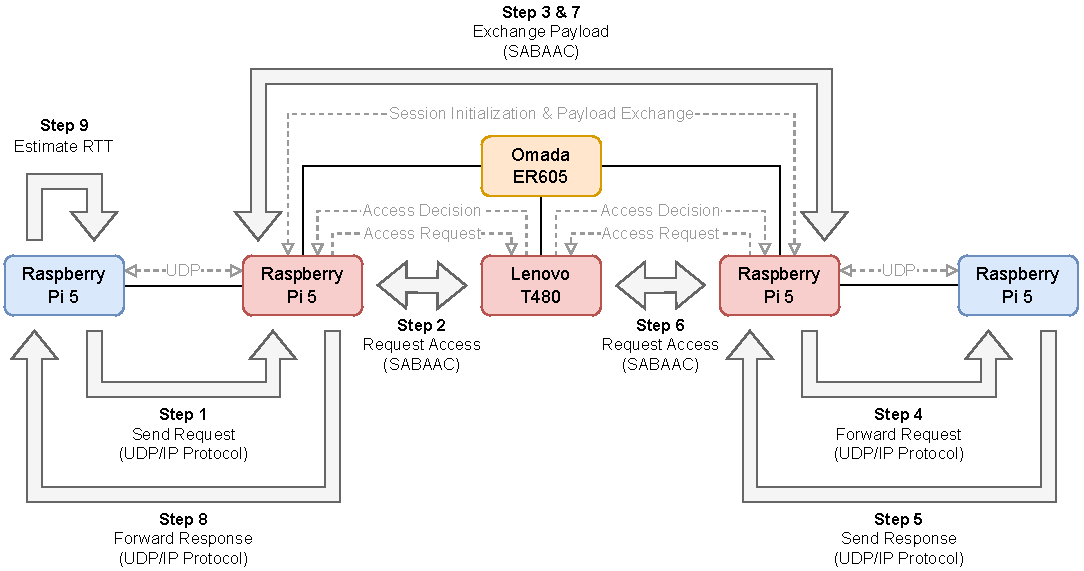
\includegraphics[width=1.0\linewidth]{figures/performance_evaluation_steps.drawio.pdf}
    \caption{Sequence of events of the experimental message exchange latency estimation.}
    \label{fig:performance_analysis_latency_steps}
\end{figure}

The results of the latency estimation experiment are shown in \autoref{tab:rtt_metrics} and \autoref{tab:rtt_share}.
The results are published open source on GitHub \cite{gitcasc} alongside the implementation of our approach.
Since CASA is an algorithm-agnostic approach, we conducted the message exchange latency estimation procedure for six different authentication algorithms.
For each of the authentication algorithms, the benchmark program sent 1000 sequential packets to estimate the RTT.
Based on the measurements, we calculated the arithmetic mean, median, standard deviation, and extrema-related values for each experiment.
Furthermore, we calculated the throughput of the PEPs in Packets Per Second (PPS), and the cumulative share of the 1000 packets in the three message types listed in \autoref{tab:message_types}.

To measure the latency offset caused by packet capturing and forwarding, we performed the initial latency estimation without authorizations, i.e., neither access control nor authentication were used.
From this data, we can see that a bidirectional message exchange between two domain entities requires 1.809 ms on average, which leads to a PEP throughput of 528.2 sequential PPS.
Without authentication, authorization, and access control in place, the measured RTTs are consistent, and each bidirectional message exchange was finished in less than 6 ms RTT, which is required to support the low latency message type.

To measure the influence of the authorization and access control, we performed a latency estimation with authorization and access control but without authentication.
For this purpose, we implemented a so-called no-operation authenticator, which processed the packets without signing or verifying them.
The measurements of the RTTs with the no-operation authenticator show that the authorization and access control workflow of SABAAC leads to an RTT increase of 1.1 ms on average.
Moreover, the increased range of minimum and maximum time indicates that SABAAC leads to an increase in RTT fluctuation.

In order to evaluate the performance of our approach in combination with symmetric cryptography, we performed a latency estimation for HMAC authentication based on SHA-512.
The results show that 99.8 \% of the message exchanges were finished in less than 6 ms RTT.
The remaining two packets or 0.2 \% of the 1000 packets satisfied the 20 ms time constraint of the medium latency message type.
By employing HMAC authentication, CASA and SABAAC achieved a throughput of 289.1 PPS at the PEPs.

To evaluate the performance of our approach in combination with PKC, we conducted latency estimations for three PKC algorithms.
For the latency estimations we chose the Ed25519 algorithm, which is an elliptic-curve digital signature algorithm, RSA-2048, and our $S_{CASA}$ signature scheme.
All three PKC approaches did not satisfy the time constraint of the low latency message type.
Ed25519 and RSA satisfied the time constraint of the medium latency message type.
$S_{CASA}$ was able to finish 99.8 \% of the message exchanges within the time constraints of the high latency message type, i.e., in less than 500 ms.
The data indicates that the RTTs of the PKC approaches are subject to fluctuations with higher magnitude compared to the fluctuations caused by SABAAC and symmetric cryptography.
Furthermore, the throughput of the PEPs was reduced by more than 70 \% compared to the HMAC authentication.
\begin{table}
    \centering
    \small
    \caption{Results of the RTT estimation based on 1000 measurements per authentication algorithm.}
    \label{tab:rtt_metrics}
    \begin{tabular}{c c c c c c c c}
    \toprule
    Authentication & Mean & Median & Deviation & \multicolumn{4}{c}{Extrema}\\
    \cmidrule(lr){5-8}
    & $\bar{x}$ & $\widetilde{x}$ & $\sigma$ & Min & Max & Range & Mid-Range\\
    \midrule
    Unauthorized    & 1.809 & 1.799 & 0.067 & 1.704 & 2.400 & 0.696 & 2.052 \\
    Unauthenticated & 2.937 & 2.924 & 0.146 & 2.808 & 4.213 & 1.405 & 3.511 \\
    HMAC            & 3.342 & 3.279 & 0.507 & 2.779 & 6.695 & 3.915 & 4.736 \\
    Ed25519        & 11.096 & 11.224& 1.591 & 9.537 & 31.971& 22.434 & 20.754 \\
    RSA-2048       & 12.703 & 12.034& 1.179 & 11.741& 16.804& 5.063 & 14.273 \\
    $S_{CASA}$    & 119.851 &113.127&28.534 &111.385&509.392&398.007&310.389\\
    \bottomrule
    \end{tabular}
\end{table}
\begin{table}
    \centering
    \small
    \caption{Throughput and cumulative message type share of the analyzed authentication algorithms.}
    \label{tab:rtt_share}
    \begin{tabular}{c c c c c}
    \toprule
    Authentication & Throughput & \multicolumn{3}{c}{Cumulative Share in Message Types}\\
    \cmidrule(lr){3-5}
     & & Low Latency & Medium Latency & High Latency\\
     & & $\leq 6~ms$ & $\leq 20~ms$ & $\leq 500~ms$\\
    \midrule
    Unauthorized    & 528.2 PPS & 1000 (100 \%) & 1000 (100 \%) & 1000 (100 \%) \\
    Unauthenticated & 328.2 PPS & 1000 (100 \%) & 1000 (100 \%) & 1000 (100 \%) \\
    HMAC            & 289.1 PPS &  998 (99.8 \%)& 1000 (100 \%) & 1000 (100 \%) \\
    Ed25519         &  88.9 PPS &    0 (0 \%)   &  998 (99.8 \%)& 1000 (100 \%) \\
    RSA-2048        &  77.4 PPS &    0 (0 \%)   & 1000 (100 \%) & 1000 (100 \%)\\
    $S_{CASA}$      &   8.2 PPS &    0 (0 \%)   &    0 (0 \%)   &  998 (99.8 \%)\\
    \bottomrule
    \end{tabular}
\end{table}

\section{Compatibility Analysis}
In this section, we conduct an analysis of the compatibility aspects of our approaches CASA and SABAAC.
The objective of the compatibility analysis is to demonstrate that our approach is a viable solution to enhance the communication security in a newly constructed or retrofitted substation.
Accordingly, the compatibility analysis serves the purpose of demonstrating that the SAS behavior and functionality is not influenced by our approach, and that SAS devices protected by CASA and SABAAC are able to provide their services and exchange information.
For this purpose, we conducted a laboratory-based experimental demonstration of applicability with industrial SAS devices.
In \autoref{sec:evaluation:compatibility:setup} the setup of the experiment is discussed.
In \autoref{sec:evaluation:compatibility:procedure} we describe the procedure and results of the experiment.

\subsection{Experimental Setup}
\label{sec:evaluation:compatibility:setup}
In total twelve devices were used to set up the experiment.
The hardware devices used for the experiment are listed in \autoref{tab:lab_hardware}.
Four of these devices were industrial SAS devices, including a MU from General Electric, an IED from ABB, an I/O box from Siemens, and a circuit breaker.
Additionally, a relay test device from Omicron was used to generate three-phase electric power, which was measured by the MU to generate SV frames.
Besides these five SAS-related devices, two Raspberry Pi 5 were used as PEPs.
A ThinkPad T480 provided the services of the PAP, PSP, PDP, and CAPP.
\begin{table}
    \centering
    \small
    \caption{Hardware used for the laboratory-based experimental demonstration of applicability.}
    \label{tab:lab_hardware}
    \begin{tabular}{c c c c c c}
    \toprule
    Manufacturer & Device & Task & SAS & CASC-SAS\\
    \midrule
    % SAS Devices
    General Electric & Reason MU320 & Process Bus Merging Unit & X & \\
    ABB & REL670 & Intelligent Electronic Device & X & \\
    Siemens & SIPROTEC 5 6MD84 & Input/Output Box & X & \\
    Hirschmann & MACH & Managed Ethernet Switch & X & \\
    Hirschmann & RSP35 & Managed Ethernet Switch & X & \\
    OMICRON & CMC 356 & Universal Relay Test Set & X & \\
    / & Circuit Breaker & Electrical Grid Switch & X & \\
    % CASA & SABAAC
    Raspberry Pi Ltd & Raspberry Pi 5 8GB & PEP & & X \\
    Lenovo & ThinkPad T480 & PDP/PAP/PSP/CAPP & & X \\
    Bechtle & ARTICONA Adapter & USB-A to RJ45 Adapter & & X \\
    \bottomrule
    \end{tabular}
\end{table}

The network topology of the devices used for the experiment is shown in \autoref{fig:lab_topology}.
In accordance with the layered SAS architecture shown in \autoref{fig:substation_architecture}, we introduced a layering of devices for the setup of the experiment.
The PAP, PSP, PDP, and CAPP were located at the bay level together with the PEP-protected IED.
As the IED only supported fiber optic network connections, we employed a Hirschmann RSP35 switch as a protocol converter.
With the protocol converter in place, the IED was connected to its PEP using Ethernet over twisted-pair.
The PEP was then connected to a Hirschmann MACH switch representing the process bus switch.
Since the Raspberry Pi 5 only possesses a single on-board RJ45 Ethernet connector, a USB-A to RJ45 Ethernet adapter had to be used for both PEPs.

At the process level of the experiment's network topology the MU was located.
The MU was connected to the relay test device using an analog connection, and was connected to the process bus switch using a fiber optic connection.
Consequently, the MU was not PEP-protected.
In addition to the MU, the PEP-protected I/O box was located at the process level, and was connected to the circuit breaker via an analog connection.
\begin{figure}
    \centering
    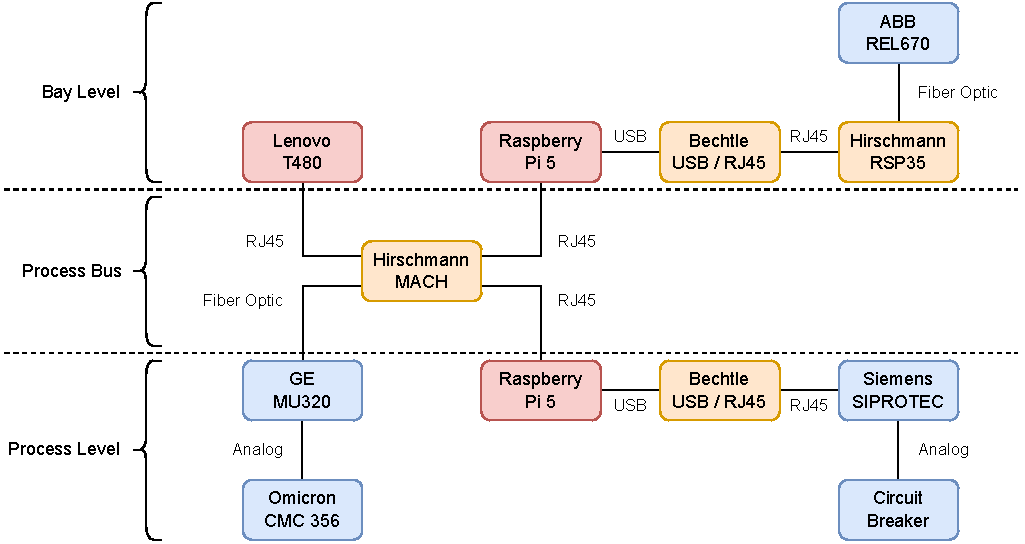
\includegraphics[width=1.0\linewidth]{figures/lab_evaluation_topology.drawio.pdf}
    \caption{Network topology of the laboratory-based experimental demonstration of applicability.}
    \label{fig:lab_topology}
\end{figure}

\subsection{Procedure \& Results}
\label{sec:evaluation:compatibility:procedure}
The procedure of the experiment comprised four key events.
The sequence of events and the corresponding messages exchanged between the devices are shown in \autoref{fig:lab_steps} and are discussed in the following:
\begin{description}
    \item[Step 1: Generate Overcurrent]~\\
    At the initial state of the experiment, the voltages and currents of all three phases generated by the Omicron CMC 356 were within certain boundaries to be detected as normal grid situation.
    Accordingly, the circuit breaker connected to the IED was closed and allowed power to flow through the grid.
    To start the experiment, we manually adjusted the generated three-phase electric power.
    The current was set to a higher level to simulate an overcurrent situation in the grid.
    This situation was communicated to the MU via a direct analog connection, i.e., the MU was measuring the voltages and currents of the three phases.

    \item[Step 2: Send Sampled Values]~\\
    The MU sampled the voltage and current values provided by the relay test device.
    The sampled values were sent to the IED using the SV protocol.
    As the MU was not protected by a PEP, we bypassed the SV frames at the IED's PEP.
    For this purpose, we programmed a static bypass rule into the IED's PEP that analyzed Ethernet frames to detect and forward SV frames sent by the MU.

    \item[Step 3: Send Trip Signal]~\\
    The IED received and processed the SV frames, and detected the overcurrent situation.
    To resolve the overcurrent situation, the IED sent a GOOSE frame to the I/O box to open the circuit breaker.
    As the IED was protected by a PEP, the outgoing GOOSE frame was captured by the PEP and processed as discussed in \autoref{sec:approach:sabaac:accesscontrol}.
    The authenticated and authorized payload exchange message, which contained the GOOSE frame, was then forwarded to the PEP of the I/O box.
    The PEP verified the incoming payload exchange message, extracted the encapsulated GOOSE frame, and forwarded the GOOSE frame to the I/O box.

    \item[Step 4: Trigger Circuit Breaker]~\\
    The I/O box received the original GOOSE frame, which was sent by the IED.
    As the GOOSE frame signalled to the I/O box to open the circuit breaker, the I/O box used an analog signal to open the circuit breaker.
    At the end of the experiment, we were able to visually verify that the circuit breaker had opened successfully.
\end{description}
\begin{figure}
    \centering
    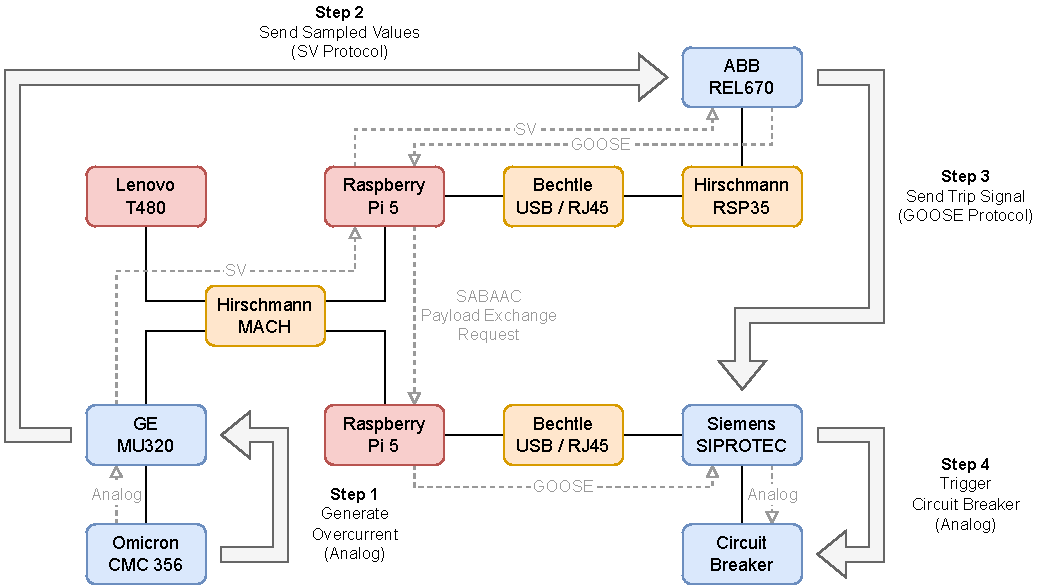
\includegraphics[width=1.0\linewidth]{figures/lab_evaluation_steps.drawio.pdf}
    \caption{Sequence of events of the laboratory-based experimental demonstration of applicability.}
    \label{fig:lab_steps}
\end{figure}

The simulated exception in the grid was successfully propagated through the SAS network during the experiment.
Consequently, the experiment demonstrated that the operation of the MU, IED, and I/O box was not disrupted by the employment of CASA and SABAAC.
Since we deployed the security-related components to inexpensive off-the-shelf hardware, we were able to demonstrate that our approach is a feasible solution for SAS environments not only security-wise and performance-wise but also cost-wise.
Due to the BITW concept of our approach, no adaptations had to be made to the SAS devices.
This indicates that our approach is a viable solution for the retrofitting of existing substations.
Furthermore, the usage of a static bypass rule in one of the PEPs suggests that incompatible or legacy devices could continue their operation in a retrofitted SAS.
Thus, the interoperability and interchangeability requirements of an IEC 61850 substation remain satisfied, while the communication security is increased by the enforcement of the CASC-SAS security policies.

\section{Discussion \& Comparison}
In this section we provide a summary of the findings of the evaluation, we contextualize our approach within the existing literature, and we describe the limitations and constraints inherent to the evaluation and our approach.
The conducted evaluation covered security, performance, and compatibility aspects of CASC-SAS, CASA, and SABAAC.
By performing a theoretical analysis of the security aspects of CASA and SABAAC, we demonstrated that our approaches are able to mitigate a set of adversarial attacks.
We proved that our signature scheme $S_{CASA}$ is existentially unforgeable under chosen-message attacks and that it resists collusion attacks under the DLP.
Furthermore, we provided definitions for message replay, forgery, modification, and time-delay attacks, and demonstrated how CASA and SABAAC interact to mitigate these attacks.
Our findings indicate that SAS devices benefit from being PEP-protected, as domain-typical DoS and false data injection attacks can be mitigated by the employment of our approach.
However, by employing CASA and SABAAC the attack surface of an SAS changes.
While IEDs, MUs, and other SAS devices benefit from being protected by using our BITW approach, the increased total number of devices in the SAS and their communication relations lead to an increased risk of DoS attacks.
In particular, the dependence on certain centralized components, such as the PDP, PAP, PSP, and CAPP, introduces new attack vectors for SAS adversaries.
Furthermore, as we conducted the security analysis theoretically, our findings might not be transferable to real SAS environments, and the behavior of CASA and SABAAC components under attack may be different from what we discussed theoretically.

In contrast to the security analysis, the performance and compatibility evaluations of our approach were conducted experimentally.
The results of both experimental evaluations suggest that CASA and SABAAC are able to secure time-critical communication in a SAS.
As we conducted the experiments using inexpensive off-the-shelf-hardware to deploy the CASC-SAS components, we demonstrated that our approach is lightweight and efficient with regard to its hardware requirements and corresponding deployment costs.
Nevertheless, the results of the performance evaluation indicate that computational performance is the primary challenge for the deployment of information security approaches in a SAS.
The findings demonstrate that lightweight yet inflexible symmetric cryptography approaches seem to be the only viable solution to secure low latency message exchanges.
However, the performance evaluation also revealed that the attribute-based authorization and access control workflows of SABAAC have only a limited impact on the overall message exchange latency.
Accordingly, the results emphasize the appropriateness of expressive and flexible yet computationally expensive access control approaches, such as ABAC, even in time and resource constrained environments.

Furthermore, the findings of the security, performance, and compatibility analysis indicate that authentication, authorization, and access control benefit from the consolidation of competencies.
Related approaches that we discussed in \autoref{ch:relatedwork}, focus on either secure communication or access control in substations.
While existing approaches for the security of SAS communication, including the BITW security filter by \citeauthor{Ishchenko2018} \cite{Ishchenko2018}, and the FPGA-based GOOSE and SV hardware encryption by \citeauthor{Rodriguez2021} \cite{Rodriguez2021}, are optimal solutions under certain circumstances, we emphasize the advantages of malleable security systems.
By integrating CASA and SABAAC into a cybersecurity and cryptography architecture for SAS, our approach enables adaption to future requirements, while it maintains a well-defined set of provided services.
In particular, our algorithm-agnostic CASA approach demonstrated the advantages of a malleable cryptography platform by supporting the employment of different algorithms for different use cases within a single SAS.

\chapter{Conclusion}
\label{ch:conclusion}
%In this last chapter, we conclude the thesis by presenting the potential future work of the proposed approach.
%The potential future work is discussed in \autoref{sec:conclusion:future_work}.
%Furthermore, in \autoref{sec:conclusion:summary}, we present a summary of the contributions and findings of the thesis.
This concluding chapter presents the potential future work of the proposed approach.
The potential future work is discussed in detail in \autoref{sec:conclusion:future_work}.
Furthermore, \autoref{sec:conclusion:summary} provides a summary of the contributions and findings of the thesis.

\section{Future Work}
\label{sec:conclusion:future_work}
% AB-PKC - Pure Cryptography
Our findings indicate that the CASC-SAS approach, its cryptographic approach CASA, and its authorization and access control approach SABAAC serve to enhance the communication security of a SAS.
In the CASC-SAS approach, the enhancement of communication security was achieved by combining cryptographic services provided by CASA with authorization and access control services provided by SABAAC.
Further research could be conducted to determine, whether this enhancement of security is also achievable by employing a purely cryptographic approach.
To answer this question, we propose the design and realization of an AB-PKC approach that satisfies the requirements of the SAS domain.
In contrast to cryptography-dependent but scheme-agnostic ABAC, as we proposed it in CASC-SAS, the AB-PKC approach could allow the accomplishment of additional security objectives, including privacy and anonymity.

% Encryption \& Decryption
In addition to the changes in the approach paradigm, further research might investigate whether the existing CASC-SAS approach could be expanded to encompass encryption and decryption in conjunction with its signing and verification operations.
While confidentiality for power systems via encryption is explicitly non-recommended for time-critical communication in the IEC standards \cite{IEC62351P6}, further research might elucidate how confidentiality can be achieved even in such time-critical systems.

% Hardware Cryptography Accelerators
With regard to the cryptographic services provided by CASA, further studies could be carried out to evaluate the advantages and disadvantages of hardware-based cryptography acceleration.
It is anticipated that the required computation time will decrease, leading to an increase in message throughput through the utilization of hardware accelerators for cryptographic algorithms.
However, factors such as algorithm compatibility, costs per acceleration unit, and computation time consistency may result in a less beneficial influence on the system than currently expected.

% NTP/PTP/ARP Support \& Time Consistency
The evaluation demonstrated that CASC-SAS is capable of securing application protocols of a SAS, as well as multipurpose transport protocols.
However, network time protocols, such as the Network Time Protocol (NTP) and the Precision Time Protocol (PTP), were bypassed by the PEP entities, as the operation of these protocols is susceptible to temporal inconsistencies resulting from authentication and access control.
Further research could investigate how network time protocols could benefit from being processed by a PEP and what additional requirement and constraints have to be satisfied with regard to computation performance and time consistency.
Moreover, lower-layer network management protocols, such as the Address Resolution Protocol (ARP), were bypassed since these protocols provide services not only to SAS devices but also to auxiliary intermediate devices, including network switches and routers.
Future studies could evaluate the feasibility of CASC-SAS to process these network management protocols and mitigate attacks related to them.

% Redundancy Protocols
Furthermore, future studies could investigate the impact of redundancy protocols in time-critical networks on the operation of our approach.
To this end, CASC-SAS could be deployed and assessed in systems utilizing the Parallel Redundancy Protocol (PRP) or Media Redundancy Protocol (MRP).

% Implementation of CASC-SAS in Switch/SDN Controller
To simplify the architectural complexity of CASC-SAS, reduce the overall costs of deployment, and enable processing of the above-mentioned network protocols, we propose the integration of CASC-SAS into network switches as an alternative realization approach.
For this purpose, further research could investigate the potential of realizing CASC-SAS through the use of Software-Defined Networking (SDN) solutions.
This SDN-based CASC-SAS could aggregate the tasks of multiple PEPs by deploying a virtual PEP for each port of a network switch.
Furthermore, distributed SDN controllers might provide the PAP, PSP, PDP, and CAPP services.

% AI for Policy Management
While the proposed PAP entities provide policy management services for human operators, future research could investigate how CASC-SAS might benefit from the utilization of artificial intelligence (AI).
The integration of AI-based intrusion detection could facilitate the creation and modification of security policies that are enforced within a SAS, thereby enabling our approach to mitigate a wider range of cyberattacks in a timelier manner.

% Deployment of CASC-SAS in Time-Critical Non-SAS Enviroments
In addition to the deployment in a SAS, further research is required to evaluate the applicability of CASC-SAS for other time-critical systems.
Therefore, we propose the evaluation of our approach in time-critical systems that have similar requirements as a SAS.
Systems that might potentially benefit from the enhanced communication security provided by our approach include industry 4.0, robotics, avionics, and medical systems.

%intra \& inter SAS communication
\section{Summary}
\label{sec:conclusion:summary}
To address the increasing relevance of cybersecurity for smart grid systems and to overcome the limitations of existing standards like IEC 62351, we proposed CASC-SAS, a novel cryptography and cybersecurity approach for SASs compliant with IEC 61850.
The two attribute-based and server-aided core concepts CASA and SABAAC represent the central parts of the four-layer dual-path CASC-SAS security architecture.

CASA provides protocols, algorithms, and schemes for PKC-based authentication, to safeguard the integrity, authenticity, and non-repudiation of SAS communication.
As a central component of the CASA approach, we proposed an algorithm-agnostic administration and processing platform, that provides key generation, key distribution, key revocation, and server-aided computation services via the proposed APEX protocol to resource-constrained devices of a SAS.
SABAAC enables the administration and enforcement of ABAC policies for time-critical and time-variable environments.
We introduced the concept of time-dependency for attributes and ABAC policies, and discussed methods to manage, distribute, and enforce such expressive and flexible but yet computationally expensive access control policies.
With regard to the management and evaluation of access control policies, this thesis proposed a delegated attribute-based authorization protocol responsible for the policy creation, management, storage, and distribution.
With regard to the enforcement of policies, we introduced a delegated attribute-based access control protocol.
To facilitate the enforcement of policies in time-critical systems, we proposed a novel policy enforcement strategy, which combines server-sided precomputation and client-sided caching of access decisions.

We implemented CASC-SAS using the object-oriented programming paradigm and the programming language Java.
The implementation is published open source on GitHub under the European Union Public Licence (EUPL).
To assess the applicability of our approach for SAS environments, we conducted a theoretical and experimental evaluation based on the implementation.
The experiments and evaluation results were published open source alongside the implementation.
Based on formal methods, the evaluation has shown that CASC-SAS is capable of enhancing the communication security of a SAS.
While SAS-typical cyberattacks can be mitigated by employing the approach, we also discussed the changed attack surface, leading to an increased risk of DoS attacks.
The evaluation demonstrated that our approach is a feasible solution for SAS environments not only security-wise but also cost-wise and due to its highly-compatible BITW concept, that allows retrofitting of existing systems.
Moreover, based on testbed-based and lab-based experiments, the evaluation demonstrated the ability of the approach to secure time-critical message exchanges.
Accordingly, CASC-SAS is capable of securing low-latency MMS, GOOSE, and SV message exchanges between the IEDs and MUs of a SAS.
\todo{TODO: GitHub/EUPL reference einfügen}
\todo{TODO: Finish summary -> Add evaluation results}

%% ---------------------------
%% |   Glossary / Acronyms   |
%% ---------------------------
% Glossary and acronyms are printed as chapter*: Used entries and non-empty chapters only!
\printglossary
\printacronyms

%% --------------------
%% |   Bibliography   |
%% --------------------

%% Add entry to the table of contents for the bibliography
\printbibliography[heading=bibintoc]

%% ----------------
%% |   Appendix   |
%% ----------------
% \appendix
% \chapter{Appendix}
\label{chap:appendix}
\section{Review Questions \& Responses}
\begin{enumerate}[label=R\arabic*.]
    \item \begin{enumerate}[label=Q\arabic*.]
        \item \textit{Unclear context of OT-related cybersecurity incidents (p. 2)} --- The context of the cybersecurity incidents was clarified by rephrasing the sentence and moving the citation to a more appropriate position.
        \item \textit{Textual citation of 3 or more authors should be shortened to et al. (p. 2 ff.)} --- The maximum number of author names in textual citations was limited to two, e.g., (Elbez, Keller, and Hagenmeyer [16]) becomes (Elbez et al. [16]).
        \item \textit{Typo in the word therefore (p. 2)} --- A missing letter was added to the word therefore.
        \item \textit{Research questions should relate to previously described challenges, and RQ1 and RQ2 should differ more from each other (p. 2)} --- All three research questions were partially reconstructed to relate to the security objectives. Moreover, the research questions were rephrased to clarify their goals.
        \item \textit{Interchanged words in contribution section (p. 3)} --- The corresponding sentence was rephrased.
        \item \textit{To which extent is the SABAAC approach flexible (p. 3)} --- Since its policies and not the approach is expressive and flexible, the sentence was rephrased. Moreover, the expressiveness, flexibility, and computationally expensiveness of the policies were further clarified.
        \item \textit{It would be good to relate the fundamentals to the field of application (p. 6)} --- Since the fundamentals were shortened from twenty to two pages, the relations between its topics and the OT/ICS/SAS-domain were lost. Moreover, the relevance of the more abstract topics including access control and cryptography for the OT-domain is not sufficiently described in the proposal. This will be added to the fundamentals chapter of the thesis, as the realization is currently an open question.
        \item \textit{A paragraph could be added to relate the related work chapter to the fundamentals (p. 7)} --- This relation is present in the long thesis proposal in the form of a division into sections, which are related to topics of the fundamentals.
        \item \textit{Please consider organizing the related work into sections (p. 7)} --- This organization is present in the long thesis proposal and will be transferred to the final master's thesis. Moreover, an extension for the cryptography-specific related work is planned.
        \item \textit{Please consider discussing some limitations of related works on ABAC and RBAC to justify the motivation of your work (p. 8)} --- The similarities and differences of the thesis and related work as well as the limitations of related work are present in the long thesis proposal.
        \item \textit{Cybersecurity and cryptography are names of CASC-SAS layers (p. 9)} --- The differences of the two layers are discussed in detail in the long thesis proposal. However, since the two words cybersecurity and cryptography are closely related, renaming or renumbering of the layers is currently under consideration.
        \item \textit{For ease of read, better present requirements as a list (p. 10)} --- In the long thesis proposal the requirements and their short descriptions are presented as a list.
        \item \textit{How does the integration of CASA effectively relate to figure 4.2 (p. 13)} --- This figure caption was shortened, and the CASA-specific part was removed for better understandability.
        \item \textit{Which adversarial attacks would be relevant as use cases (p. 16)} --- A subsection in the system model dedicated to relevant attacks and attack trees is planned for the final thesis.
        \item \textit{Which considerations would be included in the economic evaluation (p. 16)} --- Besides the aspects mentioned in the proposal, metrics such as the cost of CASC-SAS equipment will be discussed in the economic evaluation. Moreover, the economic evaluation covers the compatibility-related requirements, including interoperability and interchangeability, which are core concepts of the IEC 61850.
        \item \textit{Which evaluation aspects are possible theoretically (p. 16)} --- The theoretical evaluation covers the security proofs of CASA, the economic evaluation, and the calculation of minimum transfer time requirements for the performance evaluation. The theoretical approaches used will be discussed in detail in the corresponding evaluation sections in the thesis.
        \item \textit{Are times in the work plan total times and are increments processed in parallel (p. 17)} --- To clarify the total durations of milestones and parallel execution of increments, a sentence was added to the work plan introduction.
        \item \textit{Shouldn't software design flaws be considered before software implementation flaws (p. 20)} --- The order of the risks was changed to clarify that the design should be flawless before the implementation.
    \end{enumerate}
    \item \begin{enumerate}[label=Q\arabic*.]
        \item \textit{The figure captions are too long} --- All figure captions in the proposal were shortened.
        \item \textit{The fundamentals are lacking a cryptography section} --- A cryptography section covering symmetric and asymmetric cryptography was added to the fundamentals of the long proposal.
        \item \textit{The NIST recommendations for access control are not discussed in the fundamentals} --- A NIST recommendations section was added to the fundamentals of the long proposal.
        \item \textit{The security model of CASA makes very strong statements about EUF-CMA, which are not correct anymore} --- The strong statement was removed from the security model and the section was rephrased.
        \item \textit{The introduction chapter lacks an objective section} --- A section for the objective of the thesis was added to the introduction chapter. Moreover, the already existing research question section was integrated into the new section.
        \item \textit{The introduction chapter lacks a thesis structure section} --- A section for the proposed structure of the thesis was added to the introduction chapter of the long proposal. Moreover, a graphical representation of the structure is currently under consideration.
        \item \textit{The typical cybersecurity incidents mentioned in related work are not present in the objective of the approach} --- A paragraph for cybersecurity incidents was added to the objective section.
    \end{enumerate}
    \item \begin{enumerate}[label=Q\arabic*.]
        \item \textit{Sender and receiver are interchanged in SABAAC figures} --- The errors in the SABAAC figures were fixed.
        \item \textit{SABAAC is misspelled in the time schedule} --- The error in the time schedule figure was fixed.
        \item \textit{A deprecated security requirement is present in the CASA description in the long proposal} --- The deprecated security requirement was removed.
        \item \textit{Prof. Dr. Veit Hagenmeyer is the first examiner of the thesis} --- The examiners on the title page of the short and long proposal were changed. However, the second examiner is currently unknown.
        \item \textit{Missing group logo at title page} --- The KASTEL logo was added to the title page as group logo.
        \item \textit{Citations should be numbered in the order in which they appear} --- The ordering of the bibliography was changed.
        \item \textit{State-sponsored cybersecurity incidents included summary of incidents from 2013 to 2020 (p. 2)} --- The mentioning of non-discussed but referenced incidents from 2013 to 2020 was removed.
        \item \textit{Ordering of research questions is not consistent with main thesis focus ABAC (p. 2)} --- Changed order of RQ1 and RQ2.
        \item \textit{RQ2 and RQ3 contain concepts of contribution and shrink the solution space too much (p. 2)} --- Revised research questions by replacing concrete concepts such as certificateless and server-aided with more goal-oriented and unbiased terms such as lightweight and scalable.
        \item \textit{Introduction chapter lacks an enumeration of thesis contributions (p. 3)} --- The contribution section was rephrased and restructured. The contributions are now presented as an enumeration.
        \item \textit{The asymmetric cryptography section should be renamed to PKC and lacks a description of symmetric cryptography (p. 5)} --- The PKC section was renamed and a sentence to distinguish symmetric from asymmetric algorithms was added. The long version of the proposal contains an own section for symmetric cryptography.
        \item \textit{The economic evaluation is not possible due to missing data and the term economic/economy should be avoided (p. 16)} --- The third evaluation area was renamed to compatibility, to emphasize the new focus on interoperability and interchangeability as defined in IEC 61850, and the focus on economy in this area was reduced by rephrasing and restructuring.
        \item \textit{Overlapping increments of time schedule do not seem feasible (p. 19)} --- The realization phase was extended, and the evaluation phase was shortened by two weeks. Moreover, the increment durations and starting dates were revised to reduce overlapping phases.
    \end{enumerate}
\end{enumerate}


\end{document}
